\documentclass[11pt]{report}
\usepackage{geometry}
\geometry{hmargin=3cm,vmargin=2.5cm}
\usepackage{multicol}
\usepackage{wallpaper}
\usepackage[utf8]{inputenc}
\usepackage{graphicx,graphics}
\graphicspath{ {images/} }
\usepackage{titling}
\usepackage{fancyhdr}
\usepackage{titlepic}
\usepackage{url}
\usepackage[nottoc, notlof, notlot]{tocbibind}
\usepackage{eso-pic}
\usepackage{color}
\usepackage{eurosym}
\usepackage{setspace} 
\renewcommand{\baselinestretch}{1.5}

\begin{document}
\begin{titlepage}
	\centering
	{\scshape\LARGE IESEG SCHOOL OF MANAGEMENT \par}
	\vspace{1cm}
	{\scshape\Large Master Thesis\par}
	\vspace{1.5cm}
	{\huge\bfseries Ethereum for Investors and Stakeholders\par}
	\vspace{2cm}
	\includegraphics[width=0.5\textwidth]{Introduction/Ethereum}\par\vspace{1cm}
	{\Large\itshape Astrid Hugonin - Mathias Chicha\par}
	\vfill
	supervised by\par
	Dr.~ Paolo \textsc{Mazza}
	\vfill

% Bottom of the page
	{\large November 24, 2016\par}
\end{titlepage}
\begin{spacing}{1.0}
\chapter*{Abstract}

Satoshi Nakamoto released in 2009 the first cryptocurrency : "BitCoin"\footnote{Typography used is "Bitcoin" in this report.}. Since, more than 700 digital currencies were created, all different one from another. One of them, Ether (relying on the Ethereum network), went live in August 2015, and has become, in less than a year, the second cryptocurrency in market capitalization \cite{CRYPTOCOMPARE}. While numerous research studies have been made on the financial behavior of Bitcoin, none has today looked into the one of Ether. It is the purpose of this report.\newline

We first analyze Ether (Ethereum's crypto-asset, ETH) and define it as a commodity. We then study its hedging capabilities against the FTSE index and the Dollar, through a GARCH analysis. Our results prove that Ether has a value of hedging against the Dollar, but can not hedge against the market risk, hence fitting in portfolios of risk-seeker investors. As a continuation, we analyze Ether's correlation with Bitcoin, in order to determine the impact of having both assets in a portfolio. Our results show that they are positively correlated, hence making it risky for an investor to include both in the same portfolio. \newline

Last but not least, we determine the price drivers of Ether, by analyzing the correlation between the number of Decentralized  Applications \footnote{Distributed Applications on the Ethereum network.} in development with the price of Ether, and the relation between social media and the value of Ether. Our results show that there is a positive correlation between the number of Dapps created and Ether's value. We therefore advise investors to follow closely the development of these softwares, as it may drive the price of Ether. Regarding the correlation between social media and Ether, we analyze the number of views on Wikipedia, the number of Facebook "Talking about", the Twitter feeds and the number of Reddit post and comments per day, and find that Wikipedia, Facebook, and Reddit posts are the largest indicators of Ether's potential evolution. \newline

We recommend further research to be done on the subject once the market is a bit more mature, as recent events of Ethereum have biased our data\footnote{e.g. Structure modifications (Hard-forks) on the Ethereum network.}. Moreover, we think that a sentiment-analysis on social media may be a good advancement on the research for Ethereum.
\end{spacing}
\begin{spacing}{1.0}
{\small\tableofcontents}
\end{spacing}

\chapter*{Introduction}
\addcontentsline{toc}{part}{Introduction}

On the brink of global distrust in financial institutions, a high number of individuals are turning to alternative economy and currencies. One of them, Bitcoin, the largest cryptocurrency in terms of market capitalization, has been predominently  promoted since its creation. Bitcoin was first designed for online remittances, micropayments and commerce online, but numerous researches have proven that Bitcoin has since become a speculative good. Its properties are today closer to a synthetic commodity than to a currency\cite{SELGIN}. These characteristics brought the attention of investors and traders, who have today integrated the cryptocurrency in their portfolios. \medbreak
Due to its popularity, a lot of alternative cryptocurrencies (a.k.a. Altcoins) were developed, all with different aims. Ether, the second biggest cryptocurrency in market capitalization, which relies on the Ethereum network, is the subject of our study.\newline 
Ethereum is a protocol which enables users to develop  Decentralized Applications (Dapps) on the blockchain. These applications are distributed and do not require central authority , thus enhancing their security. Dapps are the consolidation of "smart-contracts", contracts with "if-then" scenarios, directly managed by the blockchain. Ether is the crypto-asset which serves as fuel for the smart-contracts. Consequently, Ether is the token of value of the Ethereum network, and can be traded over-the-counter. \newline
This report has for purpose to introduce stakeholders and investors to Ethereum, and to dispense recommendations on four axis for whom wants to invest in Ether.\newline
Our objective is to better identify the behaviour of Ether’s price and to assess it as an investment asset. By doing so, we address a series of recommendations regarding the integration of Ether in a portfolio and its trading. \clearpage

Our thesis follows a funnel structure: \newline
First, we introduce the concept of cryptocurrency and cover the technical details of the Bitcoin and Ethereum protocol. This introduction provides a general comprehension of the blockchain technology and its importance for decentralizated frameworks.\newline
We then discuss the definition of Ether and overview its features as a currency and as a commodity. To prove whether Ether is a currency or a commodity, we investigate its volatility and compare it to the behaviour of the US Dollar and Gold. This definition  is primordial as it allows us to easily deduct further characteristics of Ether.\newline 
Once defined, we assess Ether's capabilities as an investment asset by studying its hedging capabilities against the FTSE Index and the Dollar. As Bitcoin's market is more mature than Ethereum's,  we also compare our results with Bitcoin, in order to evaluate their similarities and try forecasting Ether's market evolution. \newline
 
On the other hand, we investigate the drivers of Ether’s price, to find the decisive factors one has to monitor. We know that Ether's value may be derived from three elements : Bitcoin, the number of Dapps on the network, and the impact of social media. We therefore chose to review these three elements and assess their influence on the value of Ether. In fact, Ether is mostly traded against Bitcoin, and it's value may thus be derived from it. This analysis serves a double purpose: it first helps us to see the hedging capabilities of Ether against Bitcoin, while measuring the influence of Bitcoin trading on Ether's value.\newline Moreover as Ether is the "fuel" required to run Dapps on the Ethereum network, we analyze the correlation between the number of Dapps with Ether's value.\newline
Eventually, as Ether has been launched not long ago, we believe that the cryptocurrency's price may be driven by social media. We review this next, overviewing the impact of Wikipedia, Facebook, Twitter and Reddit on Ether's value. \newline

However, some of our data may have been compromised due to a hack that happened on the Ethereum blockchain in June 2016, causing a huge volatility on the market and creating abnormal returns. We assess this limitation in our last chapter, by running a traditional event analysis, before dressing recommandations for further research.

\clearpage
\chapter*{Literature review}
\addcontentsline{toc}{part}{Literature review}

Ether is part of the numerous cryptocurrencies that appeared these last years such as Bitcoin, Litecoin, Monero or Ripple. The emergence of these virtual currencies is due to a new technology called the Blockchain, created to support the Bitcoin in 2009 by Satoshi Nakamoto \cite{SATOSHI}.\newline
According to a PWC definition \cite{PWC}, it is a distributed and decentralized transaction ledger, which is owned, maintained and updated by each node of the network. This network is thus based on a peer to peer system, without central authority, that monitors and manages the tokens' transaction register and verifies the correctness and truthfulness of transactions. \smallbreak
In order to maintain integrity and security, the blockchain depends on the proof-of-work concept inspired by Adam Back's Hashcash \cite{ADAM}. Computers on the network solve equations in order to validate a "block" of transactions, and each time a block is validated, it is saved on the ledger and "miners" (who solved the equation) get a reward proportional to the work they did. This process is called mining.\smallbreak
Blockchain encountered a huge success thanks to its low fees, low execution time, data efficiency and overall versatility. In fact the blockchain technology makes it possible for a group of independent parties to work with universal data sources which are automatically reconciled for all participants. Any type of data can be stored in a blockchain, from ownership of assets to contractual obligations. The most successful representative of the blockchain is a virtual currency, the Bitcoin, with \$9,636,613,130 of market capitalization \cite{CRYPTOCOMPARE}, which represents the highest capitalization on the market. \clearpage
This brought certain researchers to try to better define this cryptocurrency, and, as a matter of fact, Bitcoin became the main subject of emerging academic research literature regarding cryptocurrencies. And researchers mostly attempted to evaluate the moneyness of Bitcoin and whether it is closer to fiat money or to a commodity. \smallbreak
To be considered as a currency, Bitcoin must fulfill the three criteria of a currency: a medium of exchange, a unit of account and a store of value according to Mankiw \cite{MANKIW}. Certain  researchers think that Bitcoin doesn’t behave like a currency because of its speculative aspect\cite{VELDE}\cite{HANLEY}\cite{WILLIAMS} but also argue that Bitcoin has no intrinsic value and that its price volatility is very high, making its Dollar price vary significantly among the exchanges. Glaser \& al. \cite{GLASER} found that the majority of users treats their Bitcoin investments as speculative assets rather than as a means of payment. Consequently, Bitcoin may not become a traditional currency as it is used in too few exchanges of goods and services: according to Yermack \cite{YERMACK}, only 20 \% of all Bitcoin transactions is related to consumption. 
Besides, what differentiates Bitcoin from real currencies is its security \cite{MOORE} \cite{YERMACK}.  Bitcoin does not need a superior or central authority and cannot be controled due to its decentralized aspect. Our fiat currencies, indeed, are under the supervision of a central bank such as the FED or ECB, which guarantees their security, making Bitcoin untrustworthy.   \medbreak

On the other hand, some researchers acknowledge Bitcoin enough to consider it as a real currency - despite its virtual feature -,   betting that it could compete, on the long term with real currencies such as Dollar or Euro \cite{PLASSARAS}\cite{LUTHER}. Folkinshteyn et al. \cite{LENNON} argue that Bitcoin is an ideal medium of exchange due to the low transaction fees, as no physical location or office is required, and due to the short transaction time thanks to the mining process. Moreover, Bitcoin protocol does not take into account watch-lists or embargoed countries, and cannot restrict transfers as identities of users are unknown. Another advantage for Bitcoin is that opportunities of theft or vandalism are strongly reduced in comparison to physical currencies. \medbreak

Other researchers have investigated its similarities with a commodity. With a limited supply of 21 million, Bitcoin has a certain scarcity and liquidity limitation like other commodities. Besides, Bohme et al. [20] argue that transactions can be delayed by up to an hour due to the complexity of the calculus, hence diminishing the liquidity which is similar to precious metal. \clearpage

Another definition of Bitcoin has been given by Selgin \cite{SELGIN} who considers Bitcoin as a synthetic commodity money. As he wrote, it resembles fiat money in having no nonmonetary value; but it resembles commodity money in being not just contingently but absolutely scarce as referred in the table below. 


\begin{table}[!h]
\centering
\begin{tabular}{llccl}
                                      &                                          & \multicolumn{2}{c}{\textit{Nonmonetary Use?}}                                 &  \\
                                      &                                          & \textbf{Yes}                       & \textbf{No}                              &  \\ \cline{3-4}
\multicolumn{1}{c}{\textit{Scarcity}} & \multicolumn{1}{c|}{\textbf{Absolute}}   & \multicolumn{1}{c|}{Commodity}     & \multicolumn{1}{c|}{Synthetic Commodity} &  \\ \cline{3-4}
                                      & \multicolumn{1}{c|}{\textbf{Contingent}} & \multicolumn{1}{c|}{Coase Durable} & \multicolumn{1}{c|}{Fiat}                &  \\ \cline{3-4}
                                      &                                          & \multicolumn{1}{l}{}               & \multicolumn{1}{l}{}                     & 
\end{tabular}
\caption{Synthetic commodity definition \cite{SELGIN}}
\label{SYNTHETIC}
\end{table}

He said that it can become more effective than traditional currencies because it is capable of growing to accommodate increased money demand. Bitcoin automatically increases due to the demand but also to the mining process at a rate that will diminish in the long term to zero when the 21 millions of Bitcoin will be mined. \newline

To assess whether Bitcoin behaves like a currency or a commodity, many researches have been made on its volatility. Haudo Dyhrberg \cite{HAUDO2}significantly contributed to better understand the volatility of the Bitcoin through her GARCH and EGARCH analysis. She investigated the sensitivity of the Bitcoin’s price to macroeconomic variables and compared the results with the research done by Tully and Lucey \cite{TULLY} and Hammoudeh and Yuan \cite{HAMMOUDEH} to assess whether Bitcoin evolves like gold or Dollar. In her analysis, she includes the gold bullion USD/troy ounce rate, the CMX gold futures 100-ounce rate in USD, the Dollar-Euro and Dollar-Pound exchange rates, the Financial Times Stock Exchange Index (FTSE Index) and the Federal Funds rate. This research proves a volatility clustering and a high volatility persistence similar to gold. Besides the return of Bitcoin is more affected by the demand for Bitcoin as a medium of exchange and less by shocks which is similar to currency behaviour. Bitcoin also differs from gold because it reacts to external factors and not to endogenous factors like gold. Haudo Dyhrberg, thus, concludes that Bitcoin may be somewhere in between a currency and a commodity. She also observes that when there are positive volatility shocks to the independent variables studied, the volatility of Bitcoin’s returns decreases which makes Bitcoin preferable for risk-adverse investors. \clearpage

Haudo Dyhrberg explored the hedging possibilities of Bitcoin and assessed its capabilities in a portfolio and in risk management. Furthermore, she led a GARCH and an EGARCH analysis inspired from the studies of Baur and Lucey \cite{BAUR} on gold and Capie et al.\cite{CAPPIE} on the Dollar. Thus, to assess the hedging capabilities of the Bitcoin against FTSE and against Dollar, she analyzed the relationship between the return of the Bitcoin and the FTSE index and the relationship between the return of the Bitcoin and the Dollar-Euro exchange rate and the Dollar Sterling exchange rates.  This study showed that Bitcoin is uncorrelated with the FTSE index which proved that Bitcoin could be used to hedge against market risk similarly to gold capabilities. She also demonstrated that Bitcoin has only small positive correlations with the two exchange rates which suggests that Bitcoin can be used as a hedge against Dollar in a very short term perspective.\newline

Another study made by Ciaian, Rajcaniova, Kancs \cite{CIAIAN} attempts to better understand the volatility of Bitcoin by identifying drivers of Bitcoin’s price and how they impact its volatility. To determine the drivers, they based their research on Buchholz et al.\cite{BUCHHOLZ}, Kristoufek\cite{KRISTOUFEK} and Van Wijk’s \cite{WIJK} studies. Thus, the drivers identified are: market forces of Bitcoin supply and demand, Bitcoin attractiveness and global macroeconomic and financial development. By applying a Vector Auto Regressive (VAR) method, they discovered that Bitcoin attractiveness variables are the most important drivers of Bitcoin’s price. To measure attractiveness, Ciaian, Rajcaniova and Kancs use the total stock of Bitcoins in circulation, the volume of daily views on Bitcoin on Wikipedia, the number of new members and new posts on online Bitcoin forums.\newline

Since its launch in July 2015, Ether became the second most important capitalization on the cryptocurrencies market just after the Bitcoin. Only a very few papers have been written on Ethereum, due to its very recent launching. Nowadays, more than one year of Ether related data is available, allowing us to run a first analysis on Ether.\clearpage

Our first contribution to the literature is to assess if Ether can be considered as a currency or a commodity and what could be the drivers of Ether’s price. We discuss the capabilities of Ether to fulfill the three criteria of Mankiw and determine similarities between gold and Ether. Furthermore, we undertake the analysis of the volatility of Ether’s return by consolidating the studies that have been done on the Bitcoin and applying them to Ether. We derive our analysis from the works of Haudo Dyhrberg that we mentioned above about volatility characteristics and hedging capabilities. Then, following the work of Ciaian, Rajcaniova and Kancs, we investigate Ether’s attractiveness as a driver of its price’s returns. Eventually, we compare the results we found for Ether with Bitcoin, for all our studies.


\clearpage
\chapter*{Data}
\addcontentsline{toc}{part}{Data}
\subsection*{Sources}
In order to complete a global analysis of Ether’s price behavior this past year, we extracted several indexes, between the 30th of August 2015 (one month after the public go-live of Ethereum’s blockchain) and October 23rd 2016. The market being still very young, we focused on finding reliable hourly historical databases. We will discuss the use of the following indexes in the different chapters.\newline
 Data used in this thesis has been sourced from five different locations:\begin{itemize}
 \item Cryptocompare’s Ethereum price index \cite{CRYPTOCOMPARE}: Cryptocompare issues an index for Ether’s price, weighted from the average price of all main Ethereum exchanges. (ie: Kraken, Poloniex…) Cryptocompare also issued our data on social visibility of Ether.
 \item Ethercasts\cite{ETHERCASTS} provided us the number of Decentralized applications on the Ethereum network. 
 \item Dukascopy Forex historical data\cite{DUKASCOPY}: Dukascopy is a major swiss broker, from which we garnered our hourly foreign exchange prices: EUR/USD \& GBP/USD.
 \item Bloomberg: Bloomberg’s database was used to extract hourly and daily general indexes.
 \item Wikipedia: We retrieved from Wikipedia the number of page views per day on the "Ethereum" page.
 \end{itemize} 
\clearpage
We chose to center our study on ETH/USD exchanges, as it is today the most traded fiat currency with Ether. Ether is today mostly traded with Bitcoin\footnote{Volume chart can be found in the Appendix, Figure \ref{VOLUME}}: ETH/BTC trading allows faster transfer of funds as everything is automated. It allows user to transfer funds almost immediately from and to centralized exchanges, instead of waiting for a wire transfer confirmation. If the market shows high fluctuations, traders will be more prompt to react. The bankruptcy of Mt. Gox in February 2014 and the hack of Bitfinex in August 2016 is still in the mind of traders, who wish to have a higher control of their cryptocurrencies.\newline
Even though Bitcoin is mostly exchanged with Chinese Yen, we chose to focus on ETH/USD trading as we cannot fully assess the origin of funds for ETH/BTC exchanges. 

\subsection*{Data processing}

Retrieving data from different sources implies different structures and timelines, which all need restructuring. 
First, data from Bloomberg was flattened between the 30th of August 2015 to the 15th April of 2016, as Bloomberg doesn’t allow retrieving hourly data past six months. Followed a reprocessing from all extractions, by eliminating duplicates caused by either the change of winter time to summer time or server errors. Finally, data from Cryptocompare was adjusted to open market time, from 9am to 6pm GMT. \medbreak
Our database can be found at the following adress:\newline \url{http://bit.ly/2fuRE3e}

	
\chapter{Cryptocurrencies and Ethereum }
	\begin{flushright}
	\textit{This chapter will review the concept of decentralization and the technical aspects of Bitcoin and Ethereum, in order to provide a general comprehension of these technologies.}
	\end{flushright}
	 \section{General definition}
	The concept of decentralization and anonymity in financial transactions has been investigated since several decades, without being reached. \smallbreak
One of the first researcher on the subject, David Chaum\cite{CHAUM}, in 1983, was able to develop cryptographic transactions, thus enabling high levels of anonymity between two users, but the system, still being centralized, finished stillborn. Fifteen years later, Wei Dai presented a decentralized organization on cypherpunk's mailing list, which introduced the idea of creating money by solving computational calculations, but this idea also failed in assuring the implementation of such a process. It is in 2005, that Hal Finney, used Wei Dai’s research and proposed a "\textit{reusable proof of work}" system relying on Adam Back's Hashcash\cite{ADAM} puzzle, compensating the burdens of previous research.\newline
Finally, Satoshi Nakamoto achieved in 2009 in developing a cryptocurrency, named Bitcoin\cite{SATOSHI}, which allied all the previous research: the cryptocurrency relies on a decentralized network, where the ownership is managed through cryptographic keys, and where all transactions are monitored and approved by the network (before being saved in the Bitcoin ledger) through a proof of work protocol.\cite{BUTERIN}\newline
This Bitcoin ledger technology will later be known as the Blockchain.

	\subsection*{Decentralization through the Blockchain}
Per the Oxford Dictionary, centralization is "\textit{the concentration of control of an activity or organization under a single authority}"\cite{OXFORD}. While it is one of the oldest form of organization, centralization in banking drags users to trust third-parties, control instances or private bankers : user have no control over both their financial assets and the payment fees requested for transacting. \newline 
In fact, centralization has proven its shortcoming March 16th of 2013, when the Cypriots discovered that their bank accounts were punctuated, because of the Greek’s debt restructuration. \cite{CYPRIOTS} Since, the IMF issued a European directive who entried into force the 1st January of 2016, stating that accounts worth more than \euro 100,000 could be punctuated, if a major crisis happened\cite{HERLIN}. 
Hence, centralization leads to several known issues in the banking industry: \cite{NOIZAT}
\begin{itemize}
\item An oligopolistic market, with high barriers to entry.
\item Fraud in interest rates, by issuing interests with no economical justification.
\item No real democratic control and a "revolving doors" issue, where bankers can collude with instances of control.
\end{itemize}
The blockchain brings a consensus that liberates users from these burdens, thanks to decentralization: acting as a peer-to-peer ledger, the system is controlled by everyone who participates in the network. For Bitcoin \& Ethereum, the creation of money is not issued by accounting entries but by “miners” who support the network. For Bitcoin, the production may be compared to gold mining, where a limited supply of commodity is available (e.g. 21 million BTC), but earnable by anyone who contributes enough. As for shares in a company, the network is controlled by the person who contribute the most to the network.
\clearpage
	\subsection*{Protocol and transactions}
Bitcoin and Ethereum are the computing protocols that support the eponymous networks. A protocol is \textit"{a set of rules governing the exchange or transmission of data between devices}" \cite{OXFORD}. Famous protocols are for example SMTP (Simple Mail Transfer Protocol) for emails or HTTP (Hypertext Transfer Protocol) for the World Wide Web. For Bitcoin, the protocol allows transactions on a network which stores a decentralized and secure ledger called the Blockchain.\medbreak
A Bitcoin transaction is a message sent between two users, signed electronically with public key cryptography. In a nutshell, one user, Alice, when creating a Bitcoin wallet, issues two keys: a public and a private key. The public key is Alice’s “address”, her private key allows her to sign her messages, or to decrypt messages sent to her public address. Here, the message is a Bitcoin transaction. \newline When Bob sends Bitcoin to Alice, he sends the transaction to her public address and signs it with its own private key, ensuring that the transaction comes from his wallet. The addresses are created by an asymmetric mathematical function, that allows the user to generate a public address from the private key but not the other way around. \medbreak

\begin{figure}[!h]
\centering
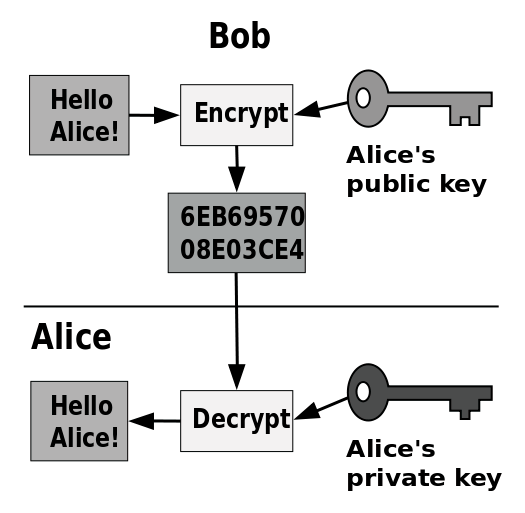
\includegraphics[scale=0.3]{Chap1/Cle}\medbreak
\caption{Asymmetric Key encryption scheme - Davidgothberg : Wikipedia}
\label{KEY}
\end{figure}

Transactions are then controlled and confirmed by the other users on the network, the miners, who save these in the Blockchain. \newline
While the mathematical signature proves who sent the transaction, it doesn't show when it was sent, and this can turn out to be problematic. \newline In our traditional banking system, if Alice wrote two checks, while not having enough money for both, the bank will accept the first check but refuse the second as her account is empty: the order of the checks is critical as it decides who gets paid. \clearpage
For Bitcoin, the order is difficult to assess  as the bank is replaced by individuals all over the world. Network delays may cause transactions to arrive in different orders and different places. Fraudsters could indeed lie about timestamps: two recipients might both think that their transactions are allowed, allowing Alice to spend her money twice. \medbreak

Transactions are hence consolidated in a pool (a block) which orders them: blocks are the recording of the number of transactions that were issued on the network since the confirmation of the last block.
\medbreak

\begin{figure}[!h]
\centering
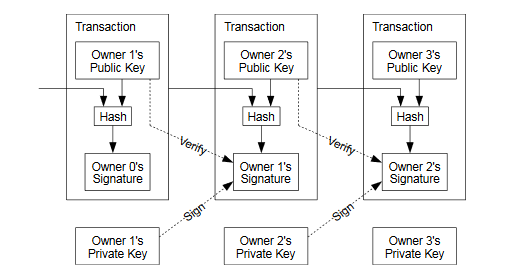
\includegraphics{Chap1/Transaction}
\caption{Simple Bitcoin Blockchain - Satoshi Nakamoto}
\label{Transaction}
\end{figure}

\medbreak
A block is the result of several hashing function, assembled as a Merkle Tree\cite{Merkle}.\newline
A hash function is defined as a function which \textit{"uses the key value of an item to compute an address for storage or retrieval of that item"}\cite{KNOTT}.\newline
In other words, it is a function which gives a unique identifier to an item. A slight variation in the input will result in an unpredictable hashed output, enhancing therefore the security of hashing functions. \clearpage
 

\medbreak
\begin{figure}[!h]
\centering
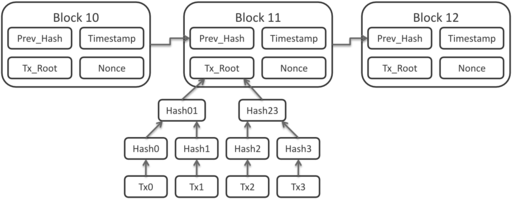
\includegraphics{Chap1/Block}
\caption{Merkle Tree in Bitcoin - Stackexchange}
\label{Block}
\end{figure}
\medbreak

A block is composed by four main different elements:
\begin{itemize}
\item A footprint of the previous block header, ensuring consistency between blocks.
\item A Unix Timestamp providing the time of the block creation.
\item A Nonce : a unique random word, which has for purpose to enhance the difficulty of the hash.
\item A Merkle Tree hash made of all transactions in the block.
\end{itemize}

A block is confirmed once a hash is found that is lower than the target fixed by the network. This target is called the difficulty, and is self-adjusted in order for a block to be mined every 10 minutes approximatively. This process of confirmation relies on the proof of work consensus.
	\clearpage
	\subsection*{Proof of work and proof of stake}
	\subsubsection*{Proof of work}
The proof of work (POW) concept was first introduced with Adam Back’s Hashcash \cite{ADAM}. This solution was developed as an answer to spamming and repeat attacks on a network. Roughly speaking, it is the solution to a lot of computational requests being sent, by engaging a cost in computation before enabling the action required, also defined as a “cost-function”. For example, in the case of e-mail spamming, the computer will need to solve an equation to validate the sending of an email. If one wants to mail-bomb, its computer calculation power required will rise accordingly to the number of emails he wants to send.\newline
In practice, the server issues a given hash, while the requester must find which word, when processed through the hash function, results in the targeted hash. Only then, the server will proceed the action requested: send an email, confirm a transaction…\newline
Adam Back’s Hashcash relies on SHA-1 functions while Satasahi Nakamoto uses SHA-256.

\medbreak
\begin{figure}[!h]
\centering
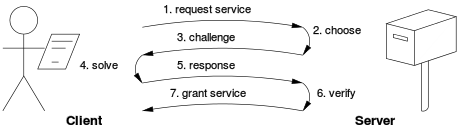
\includegraphics{Chap1/Pow}
\caption{Proof of Work illustration - Christian Faure}
\label{POW}
\end{figure}

POW for Bitcoin enables the validation of blocks in the blockchain. The process of solving the computational problem posed by the POW is called the mining, hence, the person who finds the solution are the miners. The reward for solving a block is determined by a function embedded in Bitcoin's code, equivalent to 12.5 Bitcoin for 10 minutes approximatively. Every four years, a "halving" takes place, dividing by half the remuneration of miners, in order to maintain the inflation rate. The supply rate of Bitcoin is therefore known to everyone: the last halving took place in July 2016.\newline
The POW system simultaneously shrinks the risk of hacking as the risk of malicious decision voting. By using a block structure that includes a recording of the previous block hashed, Bitcoin protects itself from attackers: if an intruder wants to modify a previous block, he will need to replicate the work done on all previous blocks and regenerate them. \newline
POW also protects the system from malicious control as the network is controlled by miners (which can be anyone/anywhere), who allocate their ressources to the network. Therefore the voting system for such a consensus depends on the involvement of miners in the network with \textit{"one-CPU-one-vote"}\cite{SATOSHI}, instead of voting through an IP adress, which could be easily spoofed. \newline
This system has however shown limitations, as Bitcoin mining farms emerged, compromising the voting system: entities having far more calculationnal power possess a greater influence on the network than others. \newline

This theory is joined with the "tragedy of the commons" scenario : once no more money bounties are be given, miners will gain only transactions fees. Since including transactions is inexpensive for miners, they will accept any transaction fee, which will gradually cause people to pay less fees, and miners to earn less money. Therefore, fewer miners will mine Bitcoin: the network difficulty will decrease, and the Bitcoin network will be more susceptible to 51\% attacks (the majority of miners hence controlling the network).\newline 
A solution discussed by the community is switching to a proof of stake system.

	\subsubsection*{Proof of stake}

Switching from Proof of Stake (POS) to POW in order to find a consensus aims to shrink the external cost of proof of work. In fact, POW is very costly in ressources: according to Adam Hayes \cite{HAYES}, the price of production of a Bitcoin is approximatively \$247.27 per BTC in March 2015. This calculation was done before the halving, and Hayes estimated that the price of production post-halving, ceteris paribus, would be of \$494.54. \newline

Concretely, the POS system works this way: a miner freezes a certain amount of cryptocurrency for a determined period (e.g. a month) by sending it in a transaction until its expiration (defined as "locktime"). In order to approve and confirm a new block, miners who possess a share in the block sign it. For pratictal reasons, a selection of these signers is randomly determined and a simple majority is required in order to approve the block. Each selected miner receives a reward from the block and can, after a while, get his participation back from the blockchain.\smallbreak
\clearpage
In theory, thanks to the random selection occuring at each block, miners can not easily corrupt the chain and have to maintain a coherent transaction history if they wish to recover their previous participation. 

\smallbreak
Proof of stake is however still highly controversial as, alone, its features are not as secure as POW's. \cite{BITFURY} A fraudster can buy private keys from corrupt individuals who participated in the creation of the early blocks. If the individual already sold his participation, he has in fact no use anymore of his private keys, and will be more keen to sell them for a bargain. The fraudster, by buying a large number of private keys will then be able to rewrite the entire transaction history in his favor. With enough keys, the hacker will have control on past and future blocks, by running the random selection process enough times until it selects a situation where he detains the majority of keys. There is therefore no more "stake" for the hacker in this consensus.

\smallbreak
In the case of Ethereum the switch from POW to POS is expected with the Casper release, but solutions for an enhanced security are still being discussed\cite{CASPER}.
\clearpage
	 \section{Ethereum and Ether}
\begin{quotation}
\quotation "\textit{The intent of Ethereum is to create an alternative protocol for building decentralized applications, providing a different set of tradeoffs that we believe will be very useful for a large class of decentralized applications, with particular emphasis on situations where rapid development time, security for small and rarely used applications, and the ability of different applications to very efficiently interact, are important.}" \newline
Vitalik Buterin, 2014 \cite{BUTERIN}
\end{quotation}
\bigbreak

By making Bitcoin’s code open-source, Satoshi Nakamoto opened the world of cryptocurrencies to many. By doing so, he ensued the emergence of many cryptocurrencies: 710 virtual currencies exist on the November 9th of 2016 \cite{CRYPTOCOMPARE}. While a numerous part of them were developed by shady developers trying to profit from the technology, some of them still distiguinshed themselves. A wide known fact is that, one of the biggest problem for the adoption of cryptocurrencies was the barrier to entry that stakeholders could face when investing in the market: a notorious scam consisted in developing a new currency, mining a proportion of its tokens, and then releasing it to the public, waiting for a price rise to happen thanks to high publicity, before “exit scamming” by selling all the tokens and abandoning the community. \medbreak

Emerged from these Altcoins Ethereum. Ethereum is a protocol designed to enhance the potential of the blockchain technology, by opening to a wider scale the use of a decentralized virtual machine (i.e. a global and worldwide computer), using a crypto-asset : Ether.
\clearpage
\subsection*{Definition}

Technically, Ethereum relies on a protocol like the one of Bitcoin. The biggest difference between Ethereum and Bitcoin lies in its blocks structure: Ethereum blocks also contain a transaction list and the latest state of the ledger’s transactions. \newline
It allows the management of two core functionalities: 

\begin{itemize}
\item Externally owned accounts (EOA): External accounts that can interact with the blockchain. In other words, a normal Ethereum address, controled by a private/public key pair.
\item Smart contracts: Contracts that were programmed to execute from the EOA if several predefined conditions are met.
\end{itemize}

These distinctions allow stakeholders to use the Ethereum network to write their own applications on the Blockchain. They are called Dapps, for Decentralized Applications, and interact through smart contracts.\newline
One of the most promising Dapp is for example Augur \cite{AUGUR} which is a decentralized prediction market. Prediction markets are today relying on centralized authorities which can be shut down or biased. By using the wisdom of the crowd \cite{SUROWIECKI} scientific principle (which implies that a group of individual tend to have more accurate predictions than one or more experts) and by rewarding users who correctly prevent future events, Augur offers a transparent system that can untie its bound from traditional prediction markets. Augur is only one amongst many Dapps: more than 200 apps exist in November 2016 per Ethercasts.\cite{ETHERCASTS} \medbreak

As Bitcoin was developed as a currency, and has a limited supply (21 Million), its value is determined by the security of its network and its scarcity, hence inheriting the surname of "digital gold". \newline 
Ether, the token of value from the Ethereum network, has its value derived from the purpose it has to execute contracts on Ethereum's network and has no limited supply. As off, it is important for investors to know that the inflation rate is therefore not controlled and that Ether as not the same consistency of Bitcoin. Ethereum's initial supply was 72 million Ether, which were sold during a public sale. Ether's remuneration for every block is five Ether. As a block is being solved every fifteen seconds approximatively, we reach an average of 18 millions Ether mined per year. This approach was decided by Ethereum's team to encourage stakeholder's to create applications on the network. \newline
\clearpage
\subsection*{The smart contracts}
\begin{quote} "\textit{
A smart contract is a computerized transaction protocol that executes the terms of a contract. The general objectives are to satisfy common contractual conditions (such as payment terms, liens, confidentiality, and even enforcement), minimize exceptions both malicious and accidental, and minimize the need for trusted intermediaries. Related economic goals include lowering fraud loss, arbitrations and enforcement costs, and other transaction costs.}" \newline
Nick Szabo, 1994\cite{Szabo}
\end{quote}

Written in Solidity, a computing language “Turing-complete” (i.e. that without theoretical limitations: everything can be calculated if the resources are appropriate), the smart contract stores rules predefined by the user, and automatically verifies them before executing the agreed terms. When the Blockchain is coupled with smart contracts it therefore removes the reliance on a central authority between the two parties, allowing a consensus where two untrusted parties can transact with each other confidently. The mechanics of a smart contract may be for example a “If-then” scenario: if A receives the payment, then A sends the goods to B. \medbreak

As stated above, the "digital oil", Ether, enables the access to the network's computational power, but does not provide any economical structure for running contracts. Therefore, "gas" was introduced as the ressource required to run contracts on the network. One "gas" is equal to 1/100,000 of Ether currently. The gas cost of a contract is proportional to the complexity of its calculations: the more ressources it requires, the more fuel will be required to run the contract. \newline 
While the network estimates a cost in gas for executing a contract, the creator of the smart contract can decide of the sum of gas he wants to spend for the execution of the contract. Miners then decide if the contract is worth its price and execute it. This function also enhances the network security from Distributed Denial of Service attacks, by making attacks costly to trigger.
\clearpage
\subsection*{DAOs and the case of "The DAO"}

While smart contracts on their own bring interest, their full potential is only unlocked when consolidated. The consolidation of these contracts can form so-called distributed autonomous agents (DAA) and decentralized autonomous organizations (DAO). Buterin envisions DAAs to be "\textit{a series of contracts that can be charged with decision-making}", while "\textit{DAOs are closer to historical business structures, allowing users to join, exercise voting power and even eventually exit such collaborations}".\cite{COINDESK}

One of the most regrettably known Dapp is "The DAO", which went live on April 30th, 2016, after 28 days of crowdfunding. \cite{DAO}\footnote{Even though it has the same name as the concept, it is important to underline that the name was chosen after the DAO concept, and that it is an independant project.}\newline 
The DAO is a decentralized governance program, which entirely relies on Ethereum. Therefore, the DAO is transparent: every action on the network is public, as are the exchanges between each user. \newline
The DAO's purpose is to enable anyone to create or participate on projects relying on the Ethereum blockchain. In other words, it is a decentralized platform for crowdfunding, and could be compared to a decentralized investment fund. None controls the platform, only safeguards are elected (called curators) who review and audit the code of projects proposed to the DAO. \newline
In order for stakeholders to vote, they have to invest in DAO Tokens, which represent the stake users have in the Dapp. Tokens embody proportionally the decision power holders have on projects. For this sake, investors can either buy directly voting assets from exchanges, or convert their Ether into tokens. If they choose this method, Ether is sent to a smart contract that automatically converts Ether to DAO tokens. 
\newline
Unfortunately, this last feature caused a breach in The DAO. On June 17th, 2016, 49 days after the go-live, a hacker drained more than 3.6 million Ether from The DAO. The hacker used maliciously a smart contract from the DAO by "splitting"\footnote{Function that transforms DAO tokens into Ether.} redudantly. As a result, Ether's value dropped from \$ 20 to approximatively \$ 13. \clearpage
Ensued a rupture in the community: On one side, partisants who believed that the "code is law", and that if the code was designed as is, the hack had to happen, in respect to the blockchain's immutability. This proposition was endorsed by the hacker, who stated that his actions were legal, as the code approved them.\cite{HACKER}\footnote{This message must be taken with precaution, as some individuals say that his cryptographic signature isn't valid.} \newline
On the other side, a community, which included Ethereum's core developpers, clearly condamned the actions of the hacker. They offered as a solution a "hard-fork" for the blockchain : the hard-fork consists in canceling all blocks issued from the hack and develop a new blockchain from this date, thus allowing users to recover their DAO Tokens. The hard-fork was approved and went live on July 20th, 2016.\newline
Since, two blockchains for Ethereum exist. The ancient one, unmodified since the hack, and the forked one. The tokens for the unmodified one are called Ether Classic (ETC) while the ones of the forked blockchain are still named Ether (ETH). Developers of Dapps already stated that they will continue to support the forked network.
\newline

While this major event opposed two interesting philosophies, we must underline the fact that even though the development of smart-contracts can be a driver of Ethereum's value, one must not forget that they may be hackable, adding an unknown and random factor to Ether's value. 



\clearpage
\chapter{Is Ether a currency or a commodity?}


	\textit{To better trade Ether, it is important to know and understand its behaviour as an asset class. \newline The cryptocurrency market is quite new and only Bitcoin has been the subject of studies, leading to a rather vague definition. The purpose of this chapter is to define Ether as a currency, a commodity or a synthetic commodity.}

	\section{Discussion about the features of Ether}
\subsection*{Can Ether be a currency?}

At first sight, virtual currencies distinguish themselves from traditional currencies, which are in physical form and controled by a central authority. The cryptocurrencies are entirely virtual and an algorithm controls the system. However, as many studies on Bitcoin have demonstrated, cryptocurrencies have many similarities with standard currency.  According to Mankiw\cite{MANKIW}, currency is defined through three main functions: a medium of exchange, a unit of account and a store of value. We use these criteria to assess if Ether can be considered as a currency.
\clearpage
\subsubsection*{Medium of exchange}

We shall identify some features which are specific to traditional currencies and make a comparison with Ether:

\textit{Transaction costs:} Ether transaction fees are lower compared to the cost of traditional means of payment such as payment by credit cards or bank transfers. The only cost needed for Ether transactions are the fee for maintaining the system, which is paid to miners. Traditional currencies have many costs linked to third-party intermediaries (banks) which perform validation, storage or security. Average transaction fees per transaction for Ether are between 0 and 1\% while traditional currencies online payments fees are between 2\%, 5\% or more\cite{TAPSCOTT}. Besides Ethereum's blockchain offers faster transaction execution than traditional payments. These characteristic may facilitate the acceptance and use of Ether as a currency. \smallbreak

\textit{Anonymity and transparency:} Ether transactions are close to anonymous and do not require personal identity information. This feature can make Ether used for illegal trades such as narcotic trades or tax evasion. Furthermore, as this money has no nationality, it makes it easier to do international transfers, which can allow tax evasion or money laundering. Another risk about “anonymity” of Ether is gambling, which appears to be an area where Ether is also used as a medium of exchange. For example, Satoshi Dice is an online gambling site specialized for cryptocurrencies where there are casinos, poker or lottery games.  Authorities can not protect people from playing on these types of platforms. However, the Ethereum blockchain is transparent and public, which means that anyone can follow the chain of transactions through the traceable history contained in the blocks. It is yet complicated to trace each identity for all the transactions as you can change your key for each transaction, but this feature raises a paradox between the protection of the identity of users and the possibility to make illegal transactions. Those two characteristics are very far from our traditional currencies which are supervised by banks or central banks.\smallbreak

 \textit{Legal tender:} Standard currencies imply a mandatory acceptance depending on countries, thus making a big difference with Ether as there is no legal tender. Businesses are not obliged to accept Ether as a means of payment for goods and services. The adoption of this cryptocurrency fully depends on its voluntary adoption by market participants. This feature can be a drag for Ether to be adopted as a medium of exchange and thus be considered like a real currency.\smallbreak
 
 \textit{Credit market:} Ethereum can be used to take loans but it is not regulated by banks, there is an over-the-counter market which permits people to have access to loans. This feature makes Ether comparable to a currency but, as an over-the-counter market is quite opaque, it is complicated to link people with each other. This problem can however be addressed through smart-contracts.\smallbreak
 
 \subsubsection*{Unit of account}
 
Ether should be able to measure the relative value of goods and services to serve as a unit of account. We analyze two characteristics which may make Ether differ from traditional currencies.\smallbreak
 \textit{Divisibility:} Like other cryptocurrencies, Ether is infinitely divisible, implying that prices may be quoted in four and more decimal compared to standard currencies which have only two decimal maximums. This constitutes an advantage for Ether as prices would be more accurate, but it can create confusion to consumers or businesses who are not accustomed.  \smallbreak
 
 \textit{Price volatility:} Since January 2016, Ether price shows a very high volatility which reduces the ability of Ether to serve as a unit of account. Businesses that use Ether must adjust all the time the price of their goods or services, creating confusion among customers. Besides, it asks more work to find their breakeven point as prices change all the time. \smallbreak   
 
 \subsubsection*{Store of value}
 
 One of the threat concerning Ethereum is that the absence of authority and the principle of “the code is the law” raised some insecurity. The blockchain already faced problems with The DAO, as we said in part 1. It has to proceed to fork in July 2016 to guarantee the value of Ether. \smallbreak
Ether is similar to a currency because it can be considered as a medium of exchange, despite the fact that very few businesses accept it as a means of payment, due to the barrier of divisibility. Its low transactions fees are a perk compared to traditional currencies. However, several aspects like the absence of legal tender and its high volatility are downsides to qualify Ether as a currency. These features are the same as what Ciaian, Rajcaniova and Kancs found on Bitcoin. This seems logical as both currencies are based on the same technology: the Blockchain, which allows them to be different from a standard currency.
 
	\subsection*{Can Ether be a commodity?}
	
We found the same results between Ether and Bitcoin about their moneyness characteristics. We can now compare Ether with gold to identify if it can be considered as a commodity, in concordance with what many researchers think about Bitcoin. We choose gold because this precious metal can be classed as a commodity and as a monetary asset. These two classifications can correspond to Ether. Gold is used as a commodity for the industrial productions (jewelry) but it was also used as a medium of exchange during the gold standard period. Nowadays, gold is traded on financial markets, making it an investment asset. Both assets need fixed initials costs. For gold, investments in equipment and human resources are mandatory for the extraction while for Ether, computer equipment and high level of computer knowledge are needed.\newline
Ether has some similarities with gold. Both are costly to extract and need miners. For gold it is huge businesses employing miners which look for and extract physically gold, while for Ether, miners are the person who emit new units. This system of mining implies that gold and Ether are both scarce.  Scarcity should permit gold and Ether to have intrinsic values, but they both are subject to high volatility. Besides, neither of them are controlled by an authority or a government, nor have a nationality. No authorization is mandatory to mine Ether or gold. \newline 
However, Ether can be used as a means of payment like we demonstrated above, in contrary to gold whose exchange for goods or services has been stopped for several decades. Also, according to the definition of Ether given by Vitalik Buterin, the founder, it is used to execute a smart-contract through a quantity of gas valued in Ether. This cryptocurrency can be considered as a commodity to consume in order to produce smart-contracts. \smallbreak

Ether is similar to a commodity, like gold in particular, as they share common features like scarcity, mining and volatility. These features make Ether difficult to define, as it both has features of commodities and currencies. By this first discussion, we think that the best definition for Ether is Selgin’s synthetic commodity money \cite{SELGIN}. To confirm this hypothesis, we will analyze the volatility of Ether in the next parts.    
\clearpage	
	\section{Data and econometric modelling}

It is complicated to link Ether to a particular asset class between currencies and commodities. We know that Ether’s price is very volatile and studying if it reacts to the same variables as the Dollar or the gold price could reveal more about the definition we can give to Ether. To do so, we apply a GARCH (Generalized autoregressive conditional heteroskedasticity) which is an econometric process to describe the volatility of a financial asset. We develop a model to assess how the returns on Ether behave compared to gold prices and to the Dollar exchange rates when analyzing the variance of these assets.\smallbreak

The data consists of intraday observations with an interval of one hour over the 08/30/2015 and 10/23/2016. We choose to study intraday data because Ether has been launched a short time ago and we want to have as many data as possible. The explanatory variable selection is based on the research of Tully and Lucey\cite{TULLY} about the sensitivities of macroeconomics variables on the price of gold. We also add the Federal Funds rate as Haudo Dyhrberg\cite{HAUDO2} did in her research on Bitcoin. The dependent variable is the returns on Ether while the independent variables are:
\begin{itemize}
 	\item Gold cash: Gold bullion USD/troy ounce rate 
 	\item Gold future: CMX gold futures 100-ounce rate in USD
 	\item EUR-USD exchange rate
 	\item GBP-USD exchange rate
 	\item FTSE index
 	\item FED fund rate
\end{itemize}

These independent variables fit with the model we want to apply because we are able to determine if the commodity market, through the gold cash and gold bullion variables, has an impact on the volatility of Ether. We also use both Dollar exchange rates, first because it is the traditional currency which is the most exchanged per day and because gold is mainly traded with Dollar. The FTSE index and the FED fund rate represents the global market which allows to identify if volatility of Ether responds to market shocks. \clearpage

The model used to investigate the similarities between Ether, gold and the Dollar is presented through the equations below. \newline
Mean and variance equations for the GARCH(1,1) model: \newline \begin{itemize}
\item $\Delta$ ln$price_t = \beta_0 + \beta_1\Delta$ ln$price_{t-1} + \beta_2 \Delta$ ln$price_{t-2} + \beta_3 \Delta$ ln$Fed_{t-1} + \beta_4 \Delta$ ln$USDEUR_{t-1} + \beta_5 \Delta$ ln$USDGBP_{t-1} + \beta_6 \Delta$ ln$FTSE_{t-1} + \beta_7 \Delta$ ln$GoldFuture_{t-1} + \beta_8 \Delta$ ln$GoldCash_{t-1} + \varepsilon_t$	
\newline
\item $\sigma_t^2 =$ exp$(\lambda_0 + \lambda_1 \Delta$ln$Fed_{t-1} + \lambda_2 \Delta$ln$USDEUR_{t-1} + \lambda_3 \Delta$ln$USDGBP_{t-1} + \lambda_4 \Delta$ln$FTSE_{t-1} + \lambda_5 \Delta$ln$GoldFuture_{t-1} + \lambda_6 \Delta$ln$GoldCash_{t-1})+ \alpha \varepsilon_{t-1}^2 + \beta_{\sigma_{t-1}^2}$
\end{itemize}\bigbreak
Where:\begin{itemize}
\item $\varepsilon_t$ determines the squared residuals.
\item $\beta$ and $\lambda$ are the coefficients.
\item $\alpha\varepsilon_{t-1}^2$ is the ARCH effect.
\item $\beta_{\sigma_{t-1}^2}$ is the GARCH effect.
\end{itemize}
\clearpage	
	\section{Methodology}

First of all, before running any analysis, we need to verify if our variables on the time period selected can fit with our models. According to Engle and Granger \cite{DING} stationary time series may lead to spurious results. Thus, to perform the model, it is necessary to have stationary series with a constant mean, variance and autovariance for each given lag. The stationarity of a series can strongly influence its behaviour and its properties. We test our variables on their stationarity thanks to the Dickey-Fuller GLS and Kwiatkowski-Phillips-Schmidt-Shin unit root tests. The number of lags we use for each variables is determined by the Akaike Information Criterion (AIC). It appears that all the variables had a unit root. The figure \ref{FIG1} confirms that Ether is sensitive to certain shocks and shows a clear non-stationarity.  To convert them into stationary data, we first process a logarithmic transformation which is insufficient.  We then, test for unit root in the first difference level which confirms the stationarity of all the variables.  \smallbreak

In the second step, we analyze the ARCH (Autoregressive Conditional Heteroskedasticity) effects. Every graph in figures \ref{FIG2} shows prolonged period of low volatility followed by periods of high volatility and vice versa. This suggests a clustering volatility, meaning that error terms are conditionally heteroskedastic and therefore can be represented by ARCH and GARCH model. The Engle’s Lagrange Multiplier \cite{GARCH} test indicated a strong ARCH effect. We verify the absence of autocorrelation hypothesis, presence of heteroscedasticity hypothesis and the normality of the errors hypothesis. Autocorrelation refers to the correlation of the time series with its own past and futures values at different points in time. \newline Usually when the datas are stationary they often reveal an absence of autocorrelation but we still tested it through the Durbin \& Watson test, hence confirming our hypothesis. The figure \ref{FIG1} shows a clear random walk which reveals heteroskedasticity. We also tested this hypothesis and confirm this feature. The third hypothesis of normally distribution of the error term was rejected, as we observe a very high kurtosis among the distribution. The error terms are rarely normally distributed so we decided to test our GARCH model despite of this problem. We admit that Ether price and the independent variables are suitable for GARCH modelling.

\medbreak
\begin{figure}[!h]
\caption{Level of Ether price, Dollar-Euro exchange rate and gold bullion rate}
\centerline{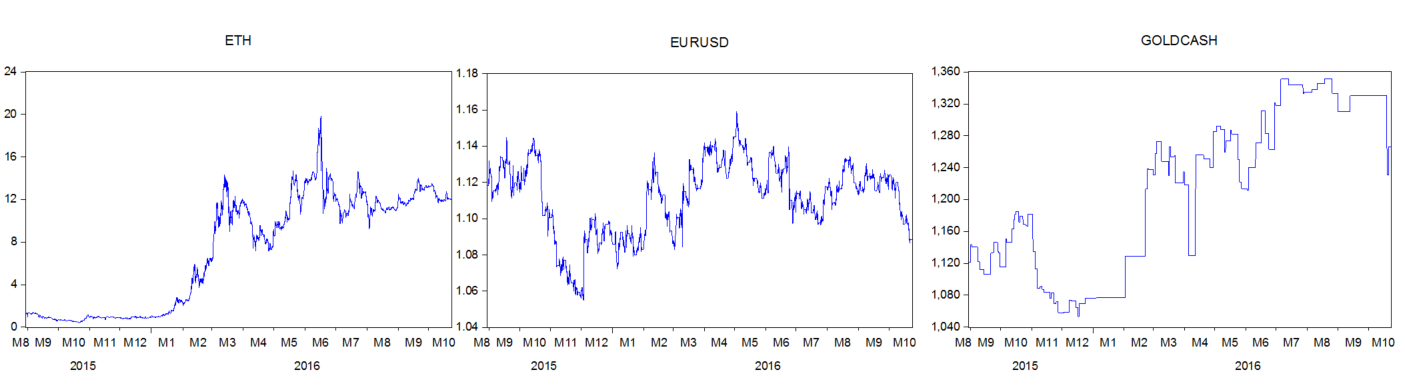
\includegraphics[scale=0.55]{Chap2/Figure1}}
\label{FIG1}
\end{figure}
\medbreak
\begin{figure}[!h]
\caption{The first differences of the logged Ether price, gold bullion rate and Dollar-Euro exchange rate}
\centerline{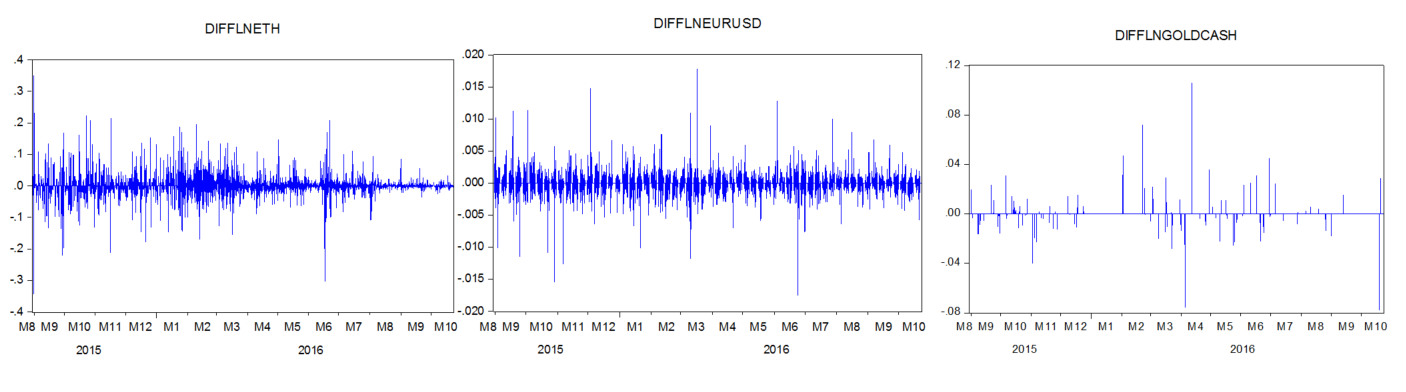
\includegraphics[scale=0.55]{Chap2/Figure2}}
\label{FIG2}
\end{figure}
\clearpage
		
\section{Results}

\begin{table}[!h]
\centering
\begin{tabular}{lllll}
\hline
\multicolumn{1}{|c|}{Variable} & \multicolumn{1}{|c|}{Coefficient} & \multicolumn{1}{|c|}{Std. Error} & \multicolumn{1}{|c|}{z-Statistic} & \multicolumn{1}{|c|}{Prob.} \\ \hline
                               &                                  &                                 &                                  &                            \\
GARCH                          & 2.068633                         & 0.615873                        & 3.358864                         & 0.0008                     \\
C                              & -0.001236                        & 0.000497                        & -2.484678                        & 0.0130                     \\
DIFFGBPUSD                     & -0.215508                        & 0.145140                        & -1.484825                        & 0.1376                     \\
DIFFLNEURUSD                   & -0.734728                        & 0.133905                        & -5.486942                        & 0.0000                     \\
DIFFLNFED                      & 0.109650                         & 0.002467                        & 44.44543                         & 0.0000                     \\
DIFFLNFTSE                     & -0.038575                        & 0.059579                        & -0.647470                        & 0.5173                     \\
DIFFLNGOLDCASH                 & 0.355102                         & 0.047547                        & 7.468433                         & 0.0000                     \\
DIFFLNGOLDFUTURE               & 0.165185                         & 0.066715                        & 2.475982                         & 0.0133                     \\
                               &                                  &                                 &                                  &                            \\ \hline
\multicolumn{5}{|c|}{Variance Equation}                                                                                                                             \\ \hline
                               &                                  &                                 &                                  &                            \\
C                              & 0.000146                         & 4.05E-06                        & 35.93251                         & 0.0000                     \\
RESID(-1)\textasciicircum 2    & 0.307083                         & 0.013004                        & 23.61531                         & 0.0000                     \\
GARCH(-1)                      & 0.615236                         & 0.008914                        & 69.01656                         & 0.0000                     \\
DIFFGBPUSD                     & 0.019916                         & 0.001330                        & 14.97526                         & 0.0000                     \\
DIFFLNEURUSD                   & -0.012103                        & 0.001549                        & -7.813262                        & 0.0000                     \\
DIFFLNFED                      & -7.15E-05                        & 6.75E-05                        & -1.059130                        & 0.2895                     \\
DIFFLNFTSE                     & -0.004025                        & 0.000549                        & -7.326968                        & 0.0000                     \\
DIFFLNGOLDCASH                 & 0.004100                         & 0.000839                        & 4.885209                         & 0.0000                     \\
DIFFLNGOLDFUTURE               & -0.000688                        & 0.000479                        & -1.437884                        & 0.1505                    
\end{tabular}
\end{table}
\bigbreak
With: \newline
\begin{itemize}
\item $\Delta$ln$priceETH= 2.0686 - 0.7347 \Delta$ln$EURUSD + 0.1096 \Delta$ln$Fed + 0.3551 \Delta$ln$GoldCash + 0.1651 \Delta$ln$GoldFuture - 0.0012$
\item $\sigma^2=$exp$(0.6152 + 0.0199\Delta$ln$GBPUSD – 0.0121\Delta$ln$EURUSD – 0.004\Delta$ln$FTSE \\ + 0.004\Delta$ln$GoldCash – 0.0006\Delta$ln$GoldFuture) + 0.307 + 0.0001$
\end{itemize} \medbreak

We observe that the GARCH effect is very significant for the mean equation which implies that previous days’ volatility strongly influenced Ether’s price. For the variance equation, the GARCH and ARCH effects are also very significant according to their $p$-value. The sum of the coefficients on the lagged squared error (RESID) and lagged conditional variance (GARCH) is very close to one (0.9222). This implies that shocks to the conditional variance will be highly persistent and that the own previous volatility shocks of Ether influence the variance of its price. From these results, we suppose that Ether’s price is highly volatile by nature and that it would be complicated in the future, to use this cryptocurrency as a medium of exchange. Indeed , it would be too complicated for businesses to express the price of their goods and services in Ether. This confirms what we said in our previous discussion about the price volatility and its capacity as a unit of account. \newline
Concerning the mean equation, the variables USD-GBP exchange rate and the FTSE index are not significant. As for the variance equation, it is the federal fund rate and the gold future which are not significant in our model.\newline
The federal fund rate, in the mean equation, has a huge influence (according to its $p$-value) and its positive coefficient implies that when this variable increases  Ether’s price increases. When the federal fund rate increases it reveals the implementation of a contractionary monetary policy by the Federal reserve in the United States. This type of policy implies that there is a rising inflation and asset prices are often overvalued meaning that Ether behaves like a traditional financial asset and follows the economic movement. This is totally different from what Tully and Lucey found about gold as when the federal fund rate increases, the gold price decreases. However, we observe that in the variance equation the federal fund rate is not significant, meaning that the fed rate has not a direct impact on the volatility of Ether. It might be the Dollar that has a real impact on Ether’s volatility. In a situation of a contractionary monetary policy, the money supply is reduced and the Dollar must appreciate. The coefficient for the EUR-USD exchange rate is negative, confirming a Dollar appreciation relative to Euro, when Ether’s price increases. We can say that Ether may have hedging capabilities against the Dollar. Besides, the variance behavior of Ether regarding the Dollar is similar to gold and thus to a commodity.\newline 
Regarding the Financial Times Stock Exchange index, its coefficient in the variance equation is negative which means that when there is a positive shock on the global stock market, the volatility of Ether decreases. Thus, when the financial markets are bullish, investors loose interest for Ether as return can be made on traditional markets. This is similar to what Tully and Lucey found about gold volatility. Again, Ether behaves more like a commodity.\newline 
The coefficients of the gold bullion (cash) in the mean and variance equation are positive which means that Ether behaves the same way as gold and can be affected by changes in gold price. This means that investors interpret Ether as gold. Again, we can conclude that Ether looks like more a commodity.\clearpage

All these results indicate that the return on Ether acts similarly to gold regarding the EUR-USD exchanges rate and the gold bullion. Moreover, due to its natural propensity to high volatility, we exclude the hypothesis of Ether as a medium of exchange and unit of account and thus, Ether does not behave like a currency. We denied our first hypothesis of considering Ether like is a synthetic commodity money. We can affirm that Ether can be considered as a commodity. This result falls in line with the definition given by Vitalik Buterin about the Ethereum blockchain. Ether is used as a commodity to consume in order to produce smart contracts and DAOs.


\clearpage	  
\section{Comparison with Bitcoin}
To compare Ether’s behavior with Bitcoin we use the research made by Haudo Dyhrberg\cite{HAUDO2}.\newline
According to her results, Ether and Bitcoin are different as she defines Bitcoin like something between a currency and a commodity. Her results show that the return on Bitcoin is more affected by the demand for Bitcoin as a medium of exchange and less by temporary shocks to the price which indicates similarities to a currency. We do not find the same results for Ether as the federal fund rate was insignificant for the variance equation. Moreover, she brought together the fact that if the federal fund rate increases and the Dollar appreciates, imports would increase and would stimulate the demand for Bitcoin. Her hypothesis makes Bitcoin more similar to an exchange rate than to a commodity which can explain why our results differ. However, she concludes with the same relation between Bitcoin and Dollar that the one we found between Ether and Dollar, and suggests that Bitcoin and Ether can have hedging capabilities against Dollar.\newline
Our results also differ from Haudo Dyhrberg with the FTSE index variable. She found that positive shocks to the stocks market make Bitcoin’s price increase and concludes that a bullish market situation may make investors more risk-seeker and invest in alternative assets like Bitcoin. Our study reveals the opposite, when the market is bullish, Ether’s volatility decrease, proving of a loss of interest from investors. This lets us suppose that Ether may be a tool to hedge against market risk. Our results may differ because Ether is still a recent market and investors buy Ether to compensate the decrease on global market thanks to its volatility.\smallbreak

This analysis told us that Ether is perceived like a commodity by investors and reveals some hedging capabilities. 

\chapter{Hedging capabilities of Ether}

\textit{The analysis of the financial abilities of an asset often considers the reactivity to the variance of other assets as well as the hedging capacities. We already studied the volatility in the previous part which suggests some hedging possibilities for Ether. To complete our analysis on its price’s behaviour we shall investigate if Ether is effectively a tool to hedge against Dollar and market risk and assess which place it can have in a portfolio. Thereby it will give a view of the place Ether can have in a portfolio and in risk management.}

	\section{Data and econometric modelling}
	
To assess the hedging capacities of Ether against Dollar and market risk, we take the same variables we used in the previous part: the FTSE index, the EUR-USD exchange rate and the GBP-USD exchange rate. These variables have already been transformed into stationary variables and there is no more change to make on them. 

	\subsection*{Hedge against the FTSE Index}
	
To identify if Ether can be used as hedge against global stock market, we use the GARCH model to analyze the relationship between the returns of Ether and the FTSE index. Our model is represented by the equation below:
\begin{itemize}
\item $\Delta$ln$priceETH = \beta_0 + \beta_1$ln$price_{t-1} + \beta_2 \Delta$ln$price_{t-2} +  \beta_3 \Delta$ln$FTSE_{t-1} + \varepsilon_t$

\item $\sigma_t^2 = \lambda0 + \alpha \varepsilon_{t-1}^2 + \beta_{{\sigma}_{t-1}^2}$
\end{itemize}
	
	\subsection*{Hedge against the Dollar model}
	
Again, we use the GARCH model to analyze the relationship between the return of the Ether and the EUR-USD exchange rate first. In this case, the relationship between Ether’s return and the GBP-USD exchange rate helps to identify if it can be use as an hedge against the Dollar. Our models are represented by the following equations:
\begin{itemize}
\item $\Delta$ln$priceETH = \beta_0 + \beta_1$ln$price_{t-1} + \beta_2 \Delta$ln$price_{t-2} +  \beta \Delta$ln$EURUSD_{t-1} + \varepsilon_t$

\item $\sigma_t^2 = \lambda0 + \alpha \varepsilon_{t-1}^2 + \beta_{{\sigma}_{t-1}^2}$

\item $\Delta$ln$priceETH = \beta_0 + \beta_1$ln$price_{t-1} + \beta_2 \Delta$ln$price_{t-2} +  \beta \Delta$ln$GBPUSD_{t-1} + \varepsilon_t$

\item $\sigma_t^2 = \lambda0 + \alpha \varepsilon_{t-1}^2 + \beta_{{\sigma}_{t-1}^2}$
\end{itemize}

\clearpage	
	\section{Methodology}
	\subsection*{Hedge against the FTSE Index}
	
We must renew our analysis of the ARCH effects as in this part we study Ether with FTSE index only. We lead a series of tests. Every graph in figure \ref{FIG32} shows prolonged periods of low volatility followed by periods of high volatility which suggests a clustering volatility. That means that error terms are conditionally heteroskedastic and therefore can be represented by ARCH and GARCH model. The Engle’s Lagrange Multiplier test indicates a strong ARCH effect. The absence of autocorrelation has been confirmed by the Durbin \& Watson test. The figure \ref{FIG31} shows a clear random walk which reveals heteroskedasticity but we also test this hypothesis to confirm that feature. The third hypothesis of normal distribution of the error term is rejected, as we observe a very high kurtosis among the distribution. The error terms are rarely normally distributed so we decided to test our GARCH model despite this problem. We admit that Ether’s price and FTSE index are suitable for GARCH modelling. 	
\medbreak
\begin{figure}[!h]
\caption{Level of Ether’s price and FTSE index}
\centerline{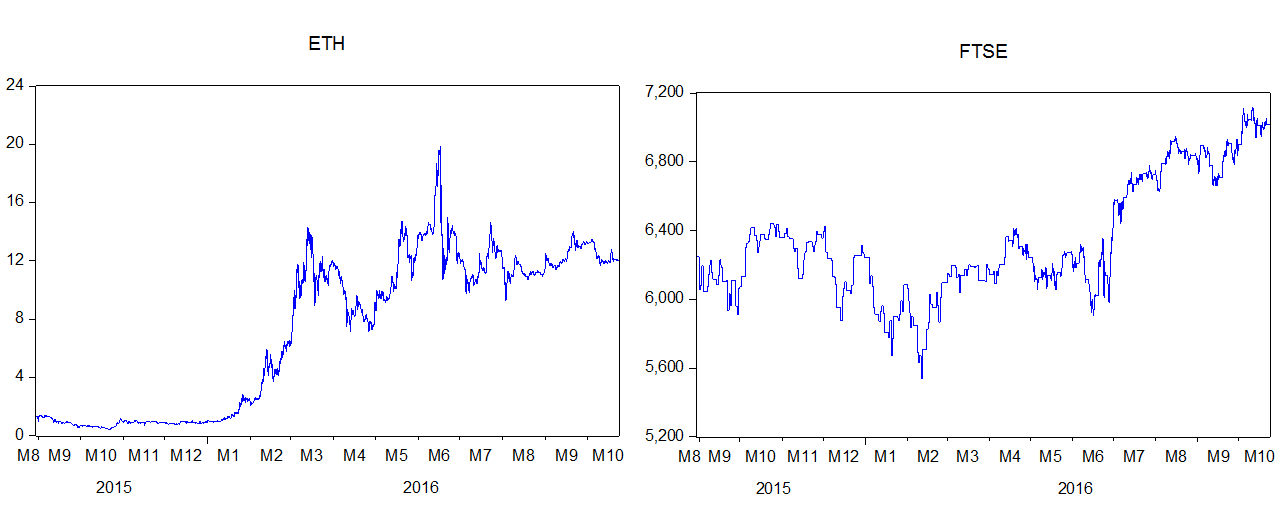
\includegraphics[scale=0.7]{Chap3/Figure1}}
\label{FIG31}
\end{figure}
\medbreak
\begin{figure}[!h]
\caption{The first difference of the logged Ether’s price and FTSE index}
\centerline{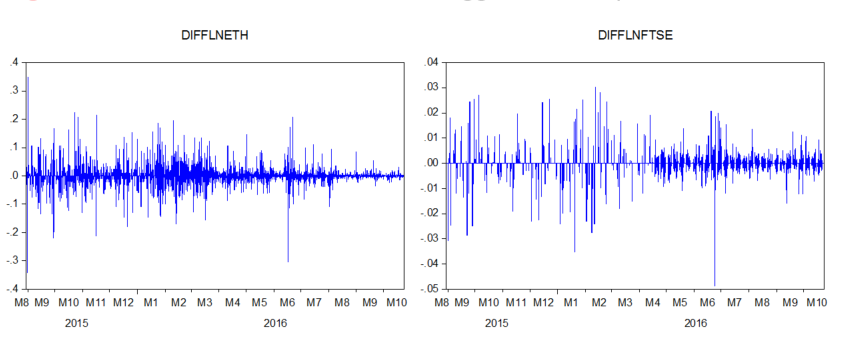
\includegraphics{Chap3/Figure2}}
\label{FIG32}
\end{figure}
\clearpage
	\subsection*{Hedge against the Dollar model}

Again, we analyze the ARCH effects for Ether and both exchange rates. The Engle’s Lagrange Multiplier test indicated a strong ARCH effect. The absence of autocorrelation hypothesis and the presence of heteroscedasticity have been confirmed. However, the hypothesis of normal distribution of the error term was rejected but we still admit that Ether’s price and the exchange rates are suitable for GARCH modelling.
\medbreak
\begin{figure}[!h]
\caption{Level of Ether’s price, EUR-USD exchange rate and GBP-USD exchange rate}
\centerline{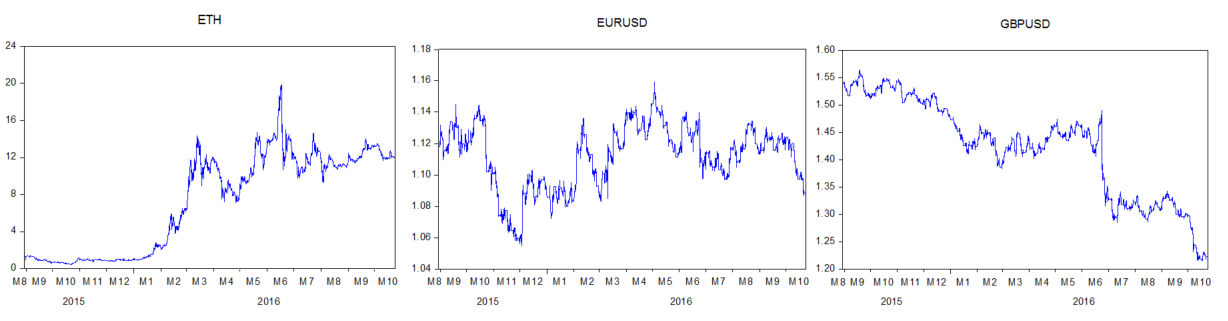
\includegraphics[scale=0.9]{Chap3/Figure3}}
\label{FIG33}
\end{figure}
\medbreak
\begin{figure}[!h]
\caption{The first difference of the logged Ether’s price, EUR-USD exchange rate and GBP-USD exchange rate}
\centerline{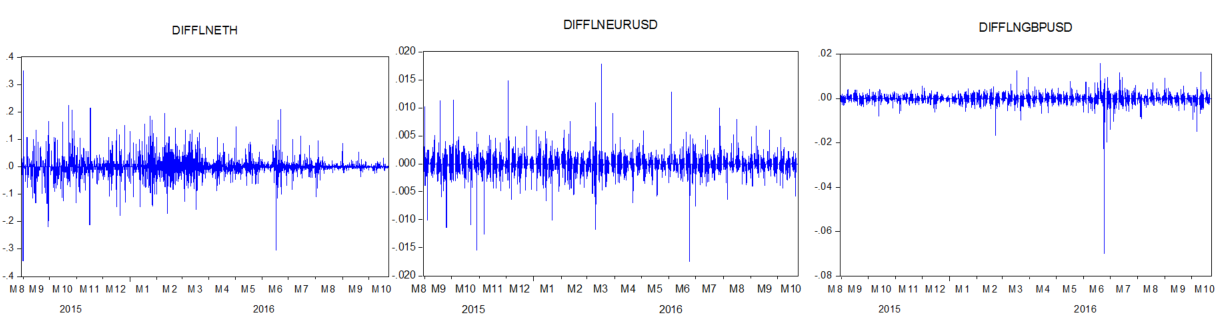
\includegraphics[scale=0.9]{Chap3/Figure4}}
\label{FIG34}
\end{figure}

\clearpage
\section{Results}
	\subsection*{Hedge against the FTSE Index}
\begin{table}[!h]
\centering
\begin{tabular}{lllll}
\hline
\multicolumn{1}{|c|}{Variable} & \multicolumn{1}{|c|}{Coefficient} & \multicolumn{1}{|c|}{Std. Error} & \multicolumn{1}{|c|}{z-Statistic} & \multicolumn{1}{|c|}{Prob.} \\ \hline
                               &                                  &                                 &                                  &                            \\
GARCH                          & 0.502943                         & 0.534936                        & 0.940193                         & 0.3471                     \\
C                              & -0.000373                        & 0.000285                        & -1.309906                        & 0.1902                     \\
DIFFLNFTSE                     & 0.386635                         & 0.047726                        & 8.101228                         & 0.0000                     \\
                               &                                  &                                 &                                  &                            \\ \hline
\multicolumn{5}{|c|}{Variance Equation}                                                                                                                             \\ \hline
                               &                                  &                                 &                                  &                            \\
C                              & 8.91E-07                         & 4.38E-08                        & 20.33562                         & 0.0000                     \\
RESID(-1)\textasciicircum 2    & 0.049324                         & 0.000964                        & 51.14483                         & 0.0000                     \\
GARCH(-1)                      & 0.958534                         & 0.000605                        & 1585.216                         & 0.0000                    
\end{tabular}
\end{table}
\bigbreak

The results show that the GARCH effect is not significant for the mean equation, whereas for the variance equation the GARCH and the ARCH effect are also very significant according to their $p$-value. The sum of the coefficients on the lagged squared error (RESID) and lagged conditional variance (GARCH) is very close to one (0.9781). This implies that shocks to the conditional variance will be highly persistent and that the own previous volatility shocks of Ether influence the variance of its price. This confirms what we found in the part on Ether’s volatility analysis. \newline
We also observe that the variable FTSE index is very significant and the coefficient is positive. Ether’s returns is affected by positive shocks on this index, meaning that when the prices of the 100 companies comprised in this index increase, Ether’s price increases. Ether thus cannot be used to hedge against market risk, contrary to the results found in the previous section. This can be explained by the fact that the coefficient is not high and this variable, in our previous model, was not significant in the mean equation. Positive shocks on FTSE index may have an indirect impact on Ether’s price. We can also defend that a bullish market situation may make investors more risk seekers and invest in alternative assets like Bitcoin. \newline
This study denied the hypothesis of hedging capabilities of Ether against market risk that we made in the previous part. This feature of Ether is different from those found in previous studies on gold. According to Baur and Lucey \cite{BAUR}, gold has hedging capabilities against stocks and market risk.  


  	\clearpage
	\subsection*{Hedge against the Dollar model}
\begin{table}[!h]
\centering
\begin{tabular}{lcccc}
\hline
\multicolumn{1}{|c|}{Variable} & \multicolumn{1}{c|}{Coefficient} & \multicolumn{1}{c|}{Std. Error} & \multicolumn{1}{c|}{z-Statistic} & \multicolumn{1}{c|}{Prob.} \\ \hline
                               & \multicolumn{1}{l}{}             & \multicolumn{1}{l}{}            & \multicolumn{1}{l}{}             & \multicolumn{1}{l}{}       \\
GARCH                          & 0.525857                         & 0.559779                        & 0.939400                         & 0.3475                     \\
C                              & -0.000337                        & 0.000304                        & -1.109571                        & 0.2672                     \\
DIFFLNEURUSD                   & -0.738162                        & 0.114322                        & -6.456889                        & 0.0000                     \\
                               & \multicolumn{1}{l}{}             & \multicolumn{1}{l}{}            & \multicolumn{1}{l}{}             & \multicolumn{1}{l}{}       \\ \hline
\multicolumn{5}{|c|}{Variance Equation}                                                                                                                             \\ \hline
                               & \multicolumn{1}{l}{}             & \multicolumn{1}{l}{}            & \multicolumn{1}{l}{}             & \multicolumn{1}{l}{}       \\
C                              & 9.53E-07                         & 3.93E-08                        & 24.24693                         & 0.0000                     \\
RESID(-1)\textasciicircum 2    & 0.047610                         & 0.001045                        & 45.57916                         & 0.0000                     \\
GARCH(-1)                      & 0.959449                         & 0.000640                        & 1499.357                         & 0.0000                     \\
\multicolumn{1}{c}{}           &                                  &                                 &                                  &                            \\
\multicolumn{1}{c}{}           &                                  &                                 &                                  &                            \\
\multicolumn{1}{c}{}           &                                  &                                 &                                  &                            \\ \hline
\multicolumn{1}{|c|}{Variable} & \multicolumn{1}{c|}{Coefficient} & \multicolumn{1}{c|}{Std. Error} & \multicolumn{1}{c|}{z-Statistic} & \multicolumn{1}{c|}{Prob.} \\ \hline
\multicolumn{1}{c}{}           &                                  &                                 &                                  &                            \\
GARCH                          & 0.514214                         & 0.556354                        & 0.924256                         & 0.3554                     \\
C                              & -0.000360                        & 0.000298                        & -1.206846                        & 0.2275                     \\
DIFFLNGBPUSD                   & -0.182866                        & 0.087985                        & -2.078375                        & 0.0377                     \\
                               & \multicolumn{1}{l}{}             & \multicolumn{1}{l}{}            & \multicolumn{1}{l}{}             & \multicolumn{1}{l}{}       \\ \hline
\multicolumn{5}{|c|}{Variance Equation}                                                                                                                             \\ \hline
                               & \multicolumn{1}{l}{}             & \multicolumn{1}{l}{}            & \multicolumn{1}{l}{}             & \multicolumn{1}{l}{}       \\
C                              & 9.87E-07                         & 3.88E-08                        & 25.41564                         & 0.0000                     \\
RESID(-1)\textasciicircum 2    & 0.048202                         & 0.000992                        & 48.60098                         & 0.0000                     \\
GARCH(-1)                      & 0.959069                         & 0.000629                        & 1525.333                         & 0.0000                    
\end{tabular}
\end{table}	
\bigbreak

The GARCH and the ARCH effect are very significant according to their $p$-value in the mean equation of our both models. The sum of the coefficients on the lagged squared error (RESID) and lagged conditional variance (GARCH) is very close to one, respectively 1.007 for EUR-USD exchange rate and 1.0072 for GBP-USD exchange rate. This implies that shocks to the conditional variance will be highly persistent and that the own previous volatility shocks of Ether influence the variance of its price in both cases. 
The results show that both exchange rates are significant variables. Their negative coefficients reveal that, when the Dollar appreciates Ether’s price increases.  Therefore, we can confirm that Ether has hedging capabilities against the Dollar. We also observe that the hedge would be more efficient against EUR-USD exchange rate because it has a quite high coefficient and GBP-USD exchange rate is less significant.\clearpage
 
This analysis confirms the hypothesis we made in the previous part about hedging capabilities of Ether against Dollar which is similar to gold capacities. Capie et al.\cite{CAPIE}, who investigated relationship between gold and Dollar noticed very small correlations between the currency and the commodity which revealed good hedging possibilities for gold against Dollar.  However, according to Baur and Lucey, gold also has abilities for hedging against market risk which is not what we find about Ether. We believe despite this feature that Ether can be considered as a commodity and can be useful in risk management. If an investor has a portfolio invested in Dollar, Ether can be a tool to hedge against a Dollar depreciation.  
 

\clearpage		
\section{Comparison with Bitcoin}

Haudo Dyhrberg \cite{HAUDO2} led the same research as we did on Bitcoin allowing us to compare between Ether and Bitcoin.\newline
Per her study, Bitcoin has hedging capabilities against market risk and Dollar. Ether is different from the Bitcoin as we found that the FTSE index affects, in a significant manner, positively the Ether’s price. Haudo Dyhrberg also used this variable but she used a different model, the threshold GARCH model with which she found a negative coefficient. Concerning the part on the volatility, we also used one of her researches and also found different results than hers on Ethereum. Our model being not so different from hers, we can conclude that Bitcoin and Ether have a different relationship with the FTSE index.   \newline
Concerning the Dollar, we found the exact same relationship between Dollar and Ether as hers with Bitcoin. Both have hedging capacities as we found very small correlation with the Dollar. Those correlations, nevertheless, reveal hedging possibilities only on a short term period. The cryptocurrencies also are more sensitive to EUR-USD exchange than to GBP-USD exchange rate. \newline

This analysis told us that Ether share some features with Bitcoin, meaning that investors on the cryptocurrencies market do not make many distinctions between Ether and the Bitcoin and trade them similarly against the Dollar. However, as Ether is a very recent cryptocurrency, a part of its volatility must be due to its launching and to the fork of July 2016 which do not permit to see clear hedging capacities against market risk unlike Bitcoin.


\chapter{Further thoughts on price drivers of Ether}
 \section{Bitcoin and Ether price correlation}
 
As Bitcoin and Ether both represent the major cryptocurrencies that exist today, one may think that they behave similarly on exchange markets. However, according to our previous analysis, Ether behaves like a commodity, contrary to Bitcoin. \newline
While both have different purposes and may therefore not have the same reaction to real life events, it is important to analyze the correlation between the two cryptocurrencies.
Bitcoin indeed has a role of "safe haven", similarly to gold, which was once again proven during the election of Donald Trump for U.S. presidency, when Bitcoin gained 3\%. Ether doesn't have this intrinsic value (as it was designed for different purposes) and seems that it's price drivers are different from the ones of Bitcoin.\newline 
This analysis is vital for an investor who wishes to integrate both cryptocurrencies in his portfolio: if both behave in a similar fashion on markets, it may not be interesting to include them in the same portfolio. \newline

Our assumptions are the following:
\begin{description}
\item[$H_0$]There is no correlation between Bitcoin and Ether.
\item[$H_1$]Bitcoin and Ether are correlated, as both are synthetic commodities.
\item[$H_2$]Ether's value derives from Bitcoin's value, as Ether is mostly traded with Bitcoin.
\end{description}

To perform this analysis, we extracted from Cryptocompare the exchange rate of both cryptocurrencies with Dollar, and ran a Pearson correlation test, as both variables are normally distributed. We chose to use daily data, from November 15th, 2015 to the 13th of November 2016. This choice is justified by the fact that we believe that the early stages of Ether trading may distort the result of our test.

The Pearson correlation formula is: \medbreak

\begin{center}
\begin{Large}
$r = \frac{\sum_{i=1}^{n}  (x_i-\bar{x})(y_i-\bar{y})}{(\sqrt{\sum_{i=1}^{n} (x_i-\bar{x})^2} \sqrt{\sum_{i=1}^{n} (y_i-\bar{y})^2}}$
\end{Large}
\end{center}

Where:
\smallbreak
\begin{itemize}

\item \begin{Large}$r$\end{Large} is the coefficient of correlation: The more it tends to -1 or 1, the more the correlation between the two datasets is strong.

\smallbreak

\item \begin{Large} $n${,} $x_i${,} $y_i$\end{Large}: $n$ is the number of values contained in both datasets. Datasets are \{$x_i$,...,$x_n$\} and \{$y_i$,...,$y_n$\}.Here $ n= 365$.

\smallbreak

\item \begin{Large} $\bar{x}= \frac{1}{n} \cdot \sum_{i=1}^{n} (x_i)$ \end{Large}: is the mean of \{$x_i$,...,$x_n$\}. 
\newline Accordingly $\bar{y}= \frac{1}{n} \cdot \sum_{i=1}^{n} (y_i)$ is the mean of \{$y_i$,...,$y_n$\}.
\end{itemize} 

 When $r$ tends to 1, it means that both variables are positively correlated, in opposition to $r$ tending to -1, where the variables are negatively correlated. A result of 0 implies that the variables are not correlated at all. \newline First, we need to overview the $p$-value of the serie. For a statistic test to be significant, its $p$-value must be  $<0.05$. Here, its value is $2,77071605515289E^{-54}$, meaning that our test is viable.\clearpage
 
Performing Pearson's correlation formula, we find that $r = 0,695874428$, which signifies that we have a strong uphill relationship between Ether and Bitcoin's value, hence confirming our \textbf{$H_1$} hypothesis and refuting \textbf{$H_0$}.
In order to answer our second hypothesis, we will now analyze $r^2$, which is equivalent to 
$r^2=0,484241220089678$. In other words, a variation in BTC has 48\% influence of Ether's value. This means therefore that Bitcoin's value has a moderate impact on Ether's price, confirming our \textbf{$H_2$}hypothesis.

\begin{figure}[!h]
\centering
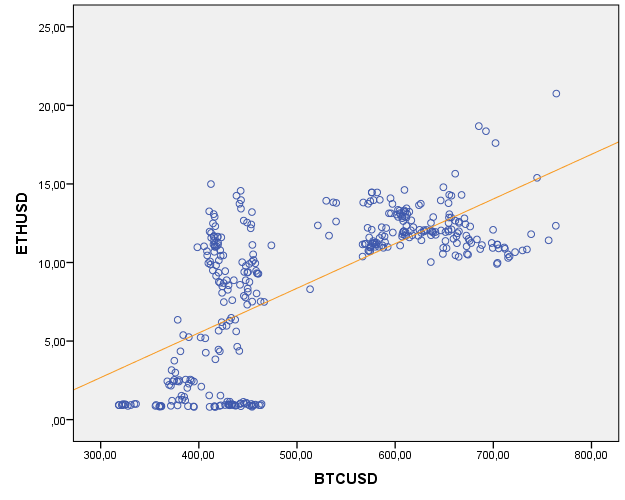
\includegraphics[scale=0.5]{Chap5/ScatterplotETHUSDBTCUSD}\medbreak
\centering
\caption{Scatter plot ETH/USD\& BTC/USD}
\label{SCATTER}
\end{figure}
\smallbreak

We suppose that due to the youth of both markets, the trust in crypto-currencies is essentially based on Bitcoin as it is the most popular. Therefore, actualities regarding Bitcoin may affect the price of Ether, as some investors may categorize them as "the same". This is a risky thought, as we already demonstrated both are solely different. Bitcoin and Ethereum must be considered as two different assets, and should not be used to hedge against each other.

\clearpage	
 \section{Decentralized applications and value of Ether}
 
 As raised in the previous chapters, the Ethereum network finds its purpose in Decentralized Applications. Ether serves as a fuel for running these applications on the network, and we believe it is important to test the correlation between the number of Dapps and Ether's value. \newline
 
 For us to run this analysis, we extracted the state of Dapps from Ethercasts\cite{ETHERCASTS}. Data from Ethercast is ranked according to the status of each project. The statuses are the following : \begin{multicols}{2}
\begin{enumerate}
 \item Unknown
 \item Abandoned
 \item On hold
 \item Stealth mode \footnote{Project currently on the test network.}
 \item Concept
 \item Work in progress
 \item Demo
 \item Working prototype
 \item Live
 \end{enumerate}
 \end{multicols}
 
 In order for us to perform an analysis using data from the previous section\footnote{i.e. from 11/15/2016 to 11/13/2016.}, we first assign a value to each Dapp depending on its status. Status 1/2/3 are each assigned the rank -1, as the state of the project could be interpretated "negatively", as for statuses 4/5/6/7/8 we assign rank 1.
As we begin our analysis from the 15th of November 2015, we begin with a base of 93 Dapps: the number of Dapps being Rank 1 at this date.\newline
 
 Our assumption is :
\begin{description}
\item[$H_1$]Ether value is highly correlated with the number of Dapps in development.
\end{description}
\clearpage
 \begin{figure}[!h]
\centering
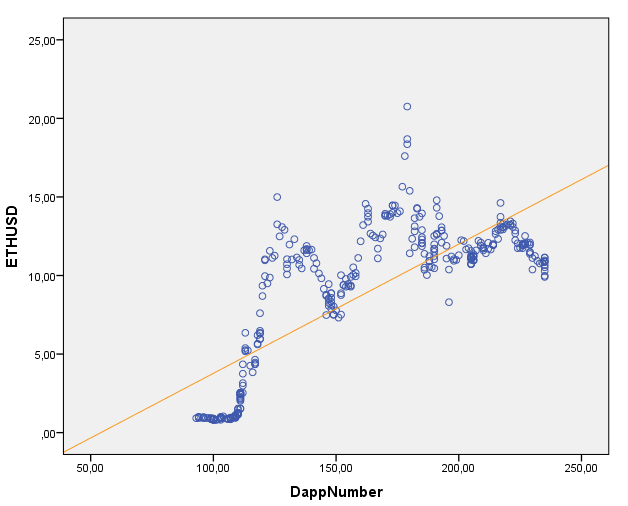
\includegraphics[scale=1]{Chap5/ScatterplotETHUSDDAPP}\medbreak
\centering
\caption{Scatter plot ETH/USD\& Number of Dapps}
\label{DAPP}
\end{figure}
\medbreak

Using Pearson's correlation model, we find the following results: 

\begin{itemize}
\item $p$-value: $4,901E^{-76}$
\item $r$: $0,780443$ 
\item $r^2$: $0,609091276249$
\end{itemize}

As the $p$-value is inferior to 0.05, we know that our correlation test is valid. The value of $r^2$ indicates that there is a strong uphill correlation between the development of Dapps on Ether's value, confirming our $H_1$ hypothesis. \newline
This results are not really surprising, as Ether is the fuel for running Dapps. According to our analysis, the more number of Dapps there will be, the more Ether will gain value. Hence, following the actualities of Ethereum development can be a good indicator on future trends of Ether.\newline 
However, this doesn't mean that one has to follow only the new projects on Ethereum. Old projects may just as much impact the value of Ether: The DAO hack is a perfect example of the bad influence that a Dapp had on Ether's price. 
In other words, do not only focus on the quantity when looking at applications, but also on the quality, past and future.
\clearpage	
 \section{Ethereum's visibility impact on Ether's price}

 While some drivers of Ether's value have been reviewed in the previous sections, we believe that social media may also influence its price. This research was done on Bitcoin by several authors \cite{SENTIMENT} \cite{BIGCOIN} and we believe it is important to adapt it for Ethereum, as both researches proved that Bitcoin was highly correlated with social media. In order to do so, we will run a multiple regression test.\newline
 
 Data used to perform this analysis has been extracted daily from Cryptocompare\cite{CRYPTOCOMPARE} and Wikipedia, and covers a year from the 14th of November, 2015. Data used are the following: \begin{itemize}
 \item ETH/USD Price
 \item Number of references of Ethereum on Facebook "Talking about" per day.\footnote{Definition from Facebook: “People Talking About This is the number of people who have created a story from your Page post.”}
 \item Number of Twitter statuses with the hashtag \# Ethereum per day.
 \item Reddit posts per day on the r/ethereum subreddit.
 \item Reddit comments per day on the r/ethereum subreddit.
 \item Number of views per day on the "Ethereum" wikipedia page.
 \end{itemize}
 
We chose to input two sources from Reddit, as it is one of the biggest discussion board on Ethereum. The choice of both posts and comments data is justified by the fact that we believe that posts may be larger price setters for Ethereum than comments. Core developers indeed post often on Reddit, and their posts may influence in a way or another the reaction of the market.\newline 
 
Hence, our hypothesis are the following:
 \begin{description}
\item[$H_1$] Ether's value is highly correlated with its visibility on internet.
\item[$H_2$] Ether's value is more correlated with Reddit than with Facebook and Twitter feeds.
\item[$H_3$]The number of views of Wikipedia pages has no impact on Ether's price.
\end{description}
\clearpage

The multiple regression formula for the Ordinary Least Square model is:\newline
$y_i = \beta_0 + \beta_1 x_i + \beta_k x_n + \varepsilon_n$ with $\beta_0$ being the intercept, $\beta_n x_n$ the regression coefficients of each dataset, and $\varepsilon_n$ the error for case $n$. \newline

First of all we need to test the multicollinearity in our data sets, in order to make it viable. Multi collinearity results show that the highest VIF  (Variance Inflation Factor) found is of 5.711 and our tolerance are all above 0.1, assuming little multicollinearity, but not an important enough one to make our test biased. The maximum threshold is of 10 \cite{BOWERMAN} for the VIF, and a minimum of 0.1 is required for the tolerance level\cite{MYERS}.  
Results of our multicollinearity analysis may be found in the appendix.\smallbreak

For our analysis, we splitted the data in three blocks, and ran our multi-regression test in a step-by-step manner. Each model containing the data from the previous block: \smallbreak

\begin{table}[!h]
\centering
\begin{tabular}{ccc}
Model 1                               & Model 2                                       & Model 3                              \\ \hline
\multicolumn{1}{|c|}{Wikipedia Views} & \multicolumn{1}{c|}{Twitter Statuses}         & \multicolumn{1}{c|}{Reddit comments} \\ \hline
\multicolumn{1}{c|}{}                 & \multicolumn{1}{c|}{Facebook "Talking About"} & \multicolumn{1}{c|}{Reddit posts}    \\ \cline{2-3} 
\multicolumn{1}{l}{}                  & \multicolumn{1}{l}{}                          & \multicolumn{1}{l}{}                
\end{tabular}
\end{table}
\medbreak
\begin{figure}[!h]
\centering
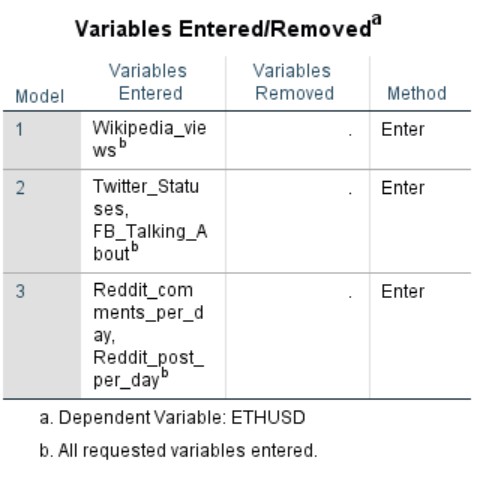
\includegraphics[scale=1]{Chap5/VariableSocial}
\caption{Models used for the multi-regression analysis}
\end{figure}
\clearpage

\subsection*{Results}
\begin{figure}[!h]
\centering
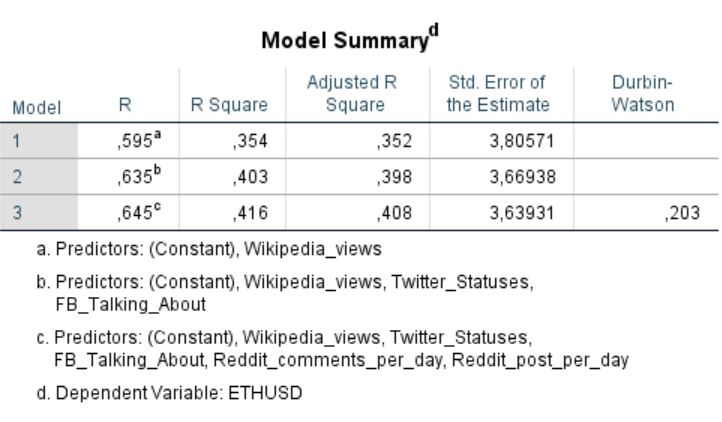
\includegraphics[scale=1]{Chap5/Modelsummary}
\centering
\caption{Ether correlation with online visibility model}
\label{Socialresults}
\end{figure}
\begin{figure}[!h]
\centering
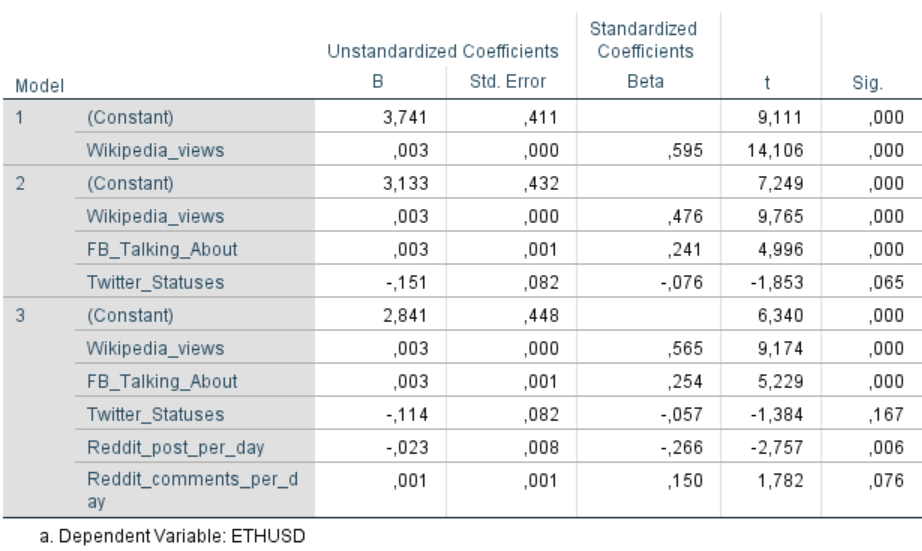
\includegraphics[scale=1]{Chap5/Coefficients}
\caption{ETH Social media - Correlation coefficients}
\end{figure}
\clearpage

The coefficient of determination, $r^2$, from the model summary table indicates that less than 50\% of the variance of Ether’s price is predictable from the independent variable we used. That means that the social medias Twitter, Facebook, Reddit and Wikipedia have a small impact on the Ether’s price volatility.\newline

This is confirmed by the significance test. In the model 1, Wikipedia is a significant variable and its coefficient is positive and average (0.595). In the model 2, we observe that Twitter is not a significant variable meaning that Twitter does not impact Ether’s price. The independent variable Wikipedia has a greater impact than Facebook. Concerning model 3, where we add the Reddit variables, Twitter is still insignificant and the Reddit comments variable is insignificant too. However, the table shows that the number of posts on Reddit about Ether is significant and has negative impact on Ether’s price while Wikipedia and Facebook still have a positive significant impact.\newline

We can therefore affirm that Wikipedia is the social media that influences the most the price of Ether. Facebook and the number of Reddit post also have an impact, but a much smaller one. We suppose that the positive impact of Wikipedia and Facebook may be induced by the word of mouth as those medias only provide explanations on Ether. Reddit posts usually provide information about the evolutions in the Ethereum’s blockchain or about the market as it was the case for the fork announcement. That could explain why this variable has a negative impact on Ether’s price. 

The only hypothesis we can therefore confirm through this analysis is $H_0$.



\clearpage
\subsection*{Independant correlation with Ether}

We also ran a Pearsons' $r$ correlation analysis on each dataset with Ether's price, in order to see if the data, ceteris paribus, could be accounted for Ether's change of value.\newline

Our results found are as follow:
\begin{figure}[!h]
\centering
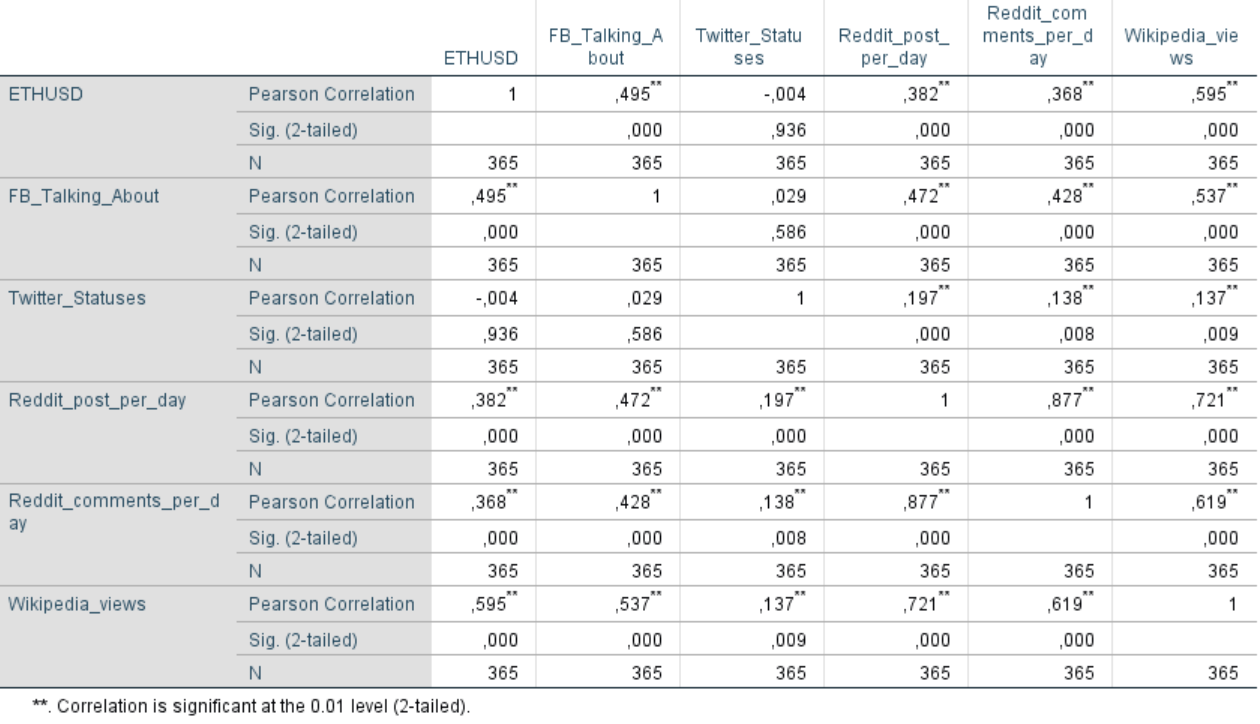
\includegraphics[scale=0.7]{Chap5/Tablecorrelation}
\caption{Correlation table : Online visibility of Ether}
\end{figure}
\medbreak

Here, only the variables of Twitter statuses are rejected as their $p$-value exceeds .05. Not surprisingly, the highest correlations found are still with the number of Wikipedia page views and the Facebook "Talking About" index. It is pretty interesting to see that Reddit posts and comments are not that significative when alone, knowing that it is one of the largest discussion board on the subject for Ethereum. \newline

While indeed following Ethereum on Reddit might be a good idea for having the latest news on the subject, we do not recommend to think that the activity on the subreddit might influence in any way the price value of Ether. We would advise to follow closely the number of views on Wikipedia pages as they better represent the voice of the silent majority.

\clearpage
\subsection*{Alternative results}
The multi-regression model used in the precedent analysis may biase results, as our data is heteroskedastic. We therefore ran another multi-regression test developed by Adam Hayes and Li Cai \cite{REGRESSION} with \textit{"heteroskedasticity-consistent standard 
error estimators"}. The most known model for this is $HC0$, but it has been proved as biased when dealing with small sample sizes. The latest, $HC4$ is the one we will use, as its characteristics suits best to our dataset, thanks to far superior small sample 
properties. \newline

Results found when running the model are: \medbreak

 \begin{figure}[!h]
\centering
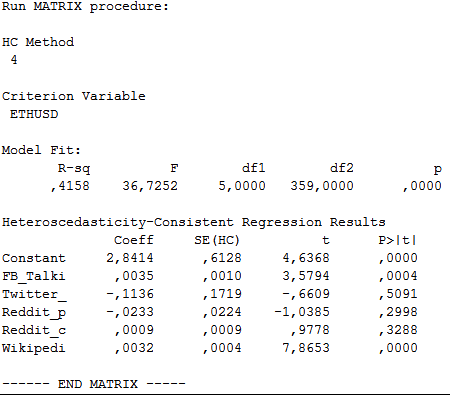
\includegraphics[scale=1.3]{Chap5/HC4}\medbreak
\centering
\caption{HC4 Method Social Media Analysis Results}
\label{HC4}
\end{figure}
\clearpage

The results when using this model are very similar from the ones found in the previous section. The $r^2$ value is .4158 which means that the model is positively correlated with Ether. In this model however, the $p$-value of Reddit Posts is significantly higher than in the previous section, hence making us reject its influence on the results. \newline
Reviewing our data through this model make us believe that only Wikipedia views and Facebook "Talking about" are influent on Ether's value, hence confirming our $H1$ hypothesis but rejecting $H2$ and $H3$. However, both correlation coefficients are really small through this model, even though the $r^2$ value is correlated. We would therefore not advise to take for granted on the long-term, the impact Facebook and Wikipedia have on Ether's value.
\clearpage

\chapter{Limitations and future work}
\section{Hard-Fork: Traditional Event analysis}
One main limitation to our analysis on the volatility of Ether is the hard-fork which happened in July 2016. As we mentioned in Chapter 1, The DAO, a Dapp on the Ethereum blockchain, was hacked on  June 17th, 2016. The hacker drained more than 3.6 million Ether from The DAO, and caused an abnormal decrease of Ether’s price from \$ 20 to approximately \$13. To solve this problem, a hard-fork solution was proposed. The announcement of this action a few days after the hack, obviously created a strong volatility on Ether’s return. \newline
The high volatility period created by this unexpected event, can have biased the result of our analysis on Ether’s volatility. To prove this assumption, we ran a traditional event analysis. To do so, we took into consideration the hack date and the hard fork date (July 22nd, 2016). We established our event window between the ten days before the hack date and the ten days after the hard-fork date. We think that the hack was not expected by the market so it should not have abnormal return before that date. The period between the hack date and the hard-fork is a period of uncertainty for investors and we think that there should have been abnormal movements on the market during this period. Besides, we chose to extend our event window to ten days after the fork date because the market had to assess the consequences of this action, which probably created an abnormal return on this period too. Concerning the estimation window, we began this period from 31 days before the hack to be sure of having a good estimation period. To examine Ether’s returns after the announcement of the hack, we compare them to Bitcoin’s return. Bitcoin is part of the cryptocurrencies market and we used it as a benchmark of the industry.

 \begin{figure}[!h]
\centering
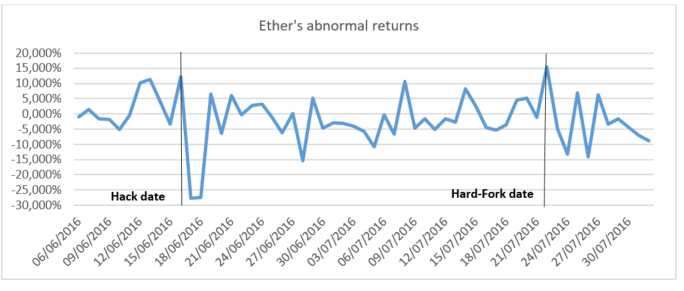
\includegraphics[scale=1.1]{Chap6/ETHAbnormal}\medbreak
\centering
\caption{Ether's abnormal returns}
\label{Abnormal}
\end{figure}
 \begin{figure}[!h]
\centering
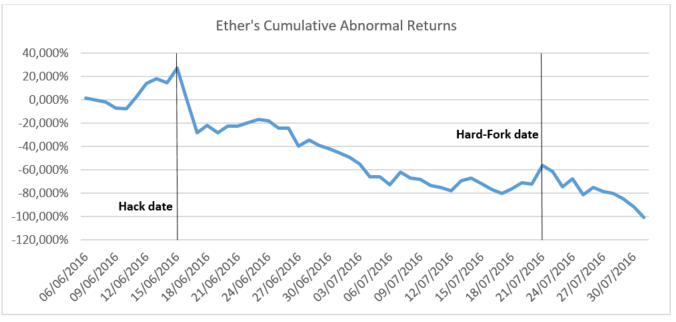
\includegraphics[scale=1.1]{Chap6/ETHCumul}\medbreak
\centering
\caption{Ether's cumulative abnormal returns}
\label{Cumul}
\end{figure}
\medbreak

From these graphs, we can clearly observe the impact of the hack and the one of the hard-fork. The amplitude Ether’s abnormal returns increases after the announcement of the both information. The figure \ref{Abnormal} shows a negative reaction of the market after the announcements. The huge volatility during this period proves the uncertainty of the market concerning the consequence of the hack and the hard-fork. The cumulative abnormal returns of Ether have a steep decrease again after both events. This indicates how these events have a negative influence on the volatility of Ether’s returns. \clearpage 
To determine if these abnormal and cumulative abnormal returns are significant, we calculate the statistic test and compare it to 1.96, which corresponds to a 5\% level of significance in the normal distribution table. The abnormal returns are significant only the day of the hack and the day after. This can be explained by natural high volatility of Ether. About the cumulative abnormal returns the results are significant as all returns after the hack and the fork are significant. However, the hack day return is not significant. This can be explained by increasing the return the day before.\smallbreak
Our results confirm our hypothesis of an abnormal volatility caused by the hack and the hard-fork. These events could have biased our previous studies on volatility of Ether and on its hedging capabilities. \clearpage

\section{Future Research}
\subsection*{A new market}
The initial stage of the Ether market and the hard-fork that created abnormal fluctuations in the market, constitute limits to our study. Indeed, the Ether market is very recent, as Ethereum's blockchain has been launched in June 2015, allowing us to study only one year of data. At its launch, Ether had not very much volatility due to a lack of notoriety that reduced our period of study. Besides, with the results we found about the abnormal return, the period covered in our study is biased. The significant data in our analysis covers only 9 out of 12 months studied, revealing that only 75\% of our total data are significant. The results we found about volatility and hedging capabilities may not reveal the real capacities of Ether as an investment tool. Thus, we suggest to test our analysis when the market will be more mature.\newline
Moreover, as proven in our study, the number of Dapp or DAOs developed through the Ethereum blockchain can influence the volatility. In the long term, the number of smart contracts and DAOs must increase as it is one of the purpose of the Ethereum blockchain, in opposition to Bitcoin. Smart contracts and DAOs can increase the productivity of businesses, and are already investigated by big companies, through the Blockchain consortium. As more companies will adopt the technology, Ether will gain more value, developing a unique market. This point is really interesting as well for investors as they can speculate, as for researchers, who will be able to analyze a new form of commodity markets.

\clearpage
\subsection*{Further in-depth social media analysis}

As seen in Chapter 4, Ether's price drivers also include social media and the visibility of Ethereum's network. However, even though our work covered main social networks over Ethereum, it would be interesting to push the analysis a little further on two points. \newline
The first one regards the visibility of Ethereum on the Internet. In fact, we believe it would be interesting to integrate data from main search engines (Google, Yahoo, Bing) in our model, but also from alternative search engines such as DuckDuckgo, as we think that the community of Ethereum use more privacy-respectful tools. Unfortunately, none of these engines allow queries on their data \footnote{Except Google, but weekly, hence biasing our model.} making therefore the analysis difficult to establish.\newline
Our second regret is the lack of data acquired on Social Media. A research led by Ifigeneia Georgoula, Demitrios Pournarakis, Christos Bilanakos,Dionisios N. Sotiropoulos, and George M. Giaglis \cite{SENTIMENT} demonstrated interesting results concerning Bitcoin's value correlation with sentiments emitted from Twitter feeds. They used Support Vector Machines in order to analyze daily tweets emitted on the platform, and proved that, in the short run, Twitter feeds and Bitcoin's price were positively correlated. Data was collected over 78 days through a web-crawler. Due to a lack of means, we weren't able to achieve such a research on Ethereum, but we invite anyone to use the following approach to analyze Ether.

\chapter*{Conclusion}
\addcontentsline{toc}{part}{Conclusion}

The aim of our paper was to define and analyze Ether, the token of value of the Ethereum blockchain. Acting as a fuel for Decentralized Applications, it was important to first define it, according to its properties. Indeed, one could consider Ether as "double hatted". On the one hand, it could have the same properties as its big brother, Bitcoin, and be a synthetic commodity. While on the other hand, it could be as oil, a commodity, as their use is similar.\newline
Our research shows that overall, Ether can be considered as a commodity. Its behavior is in fact much closer to gold than to the Dollar, as reviewed in the second chapter. It is closer to gold not only regarding its features but also with its hedging capabilities against the US Dollar. These similarities indeed made Ether inherit the surname of "digital oil", in opposition to "digital gold" for Bitcoin.\newline
We can however distinguish a difference with gold in the fact that Ether cannot be used to hedge against the market risk, according to our analysis with the FTSE Index. This allows us to conclude that Ether has its place in a portfolio, but due to its huge volatility, it would only fit with risk-seeker investors. Similarities with Bitcoin do not stop here, and as Bitcoin, Ether may be used in a portfolio in order to hedge against the Dollar. \newline

This correlation between the most known cryptocurrencies in the world may be explained by the trust people have in these technologies. Bitcoin, by representing the largest market capitalization, indicates to cryptocurrency stakeholders the health of the overall market, and may influence, in one way or another, the market of Ether, even though their public is slightly different. This being said, we therefore would not recommend integrating both of them in the same portfolio, nor to constitute a portfolio composed solely of crypto-assets.\clearpage
 
 These statements allow us to better apprehend the behavior of Ether on the market: as golds value may be influenced by the jewelry market, Ether's price must be derived from its use to create goods. In fact, gold is used to produce jewelry, and the more it is needed, the more its price tends to raise. We believe that Decentralized Applications are the equivalent of jewelry to Ether. As Ether gets "burned" when used to run an application, Ether's value may be influenced by the number of Dapps. According to our research, it is indeed the fact, as both are mildly positively correlated. This correlation can be considered as logic on the first thought, but one may not forget that these same Dapps can influence badly the market value of Ether. Indeed, a perfect and recent example is "The DAO" which showed how a Dapp impacted Ether's value due to a hack. As for any market or asset, following closely news regarding Ethereum and its development is therefore an obligatory condition for whom wants to invest in this asset.\newline
 
As Ethereum's market is recent, its value can be derived from the marketing done on the project, and therefore from its relationship with social media. One of the main places of discussion on Ethereum is Reddit's dedicated subreddit, and we believed that it was one of the most representatives of Ether's value, as developers and stakeholders both meet on the platform. However, we were largely surprised when we realized that, as seen in Chapter 4, Ether's value is mostly derived from Facebook and Wikipedia activity. 
One explanation for this could be the interest raised in newcomers for Ethereum: they invest rapidly after having heard about the technology. Another reason may be the population that composes the vocal minority.\footnote{The vocal minority, opposed to silent majority, represents users who express themselves on a given subject.} Users who discuss Ethereum on social media may not be the largest investors in the market, and could therefore not control it.\newline

Our research aims to serve as a guide for investing in Ether, by giving the reader all the keys needed for success. However, the market's youth and the DAO hack may have biased our results, as we have abnormal volatility during certain periods. In order to assess these problems, we recommend readers to renew  our study on the volatility of Ether once the market is more mature. And, as many projects are underway regarding the use of the Ethereum blockchain, we believe it will be much more interesting once Dapps become mainstream. 
\clearpage
\section*{Personal recommendations}
As final and \textit{personal} recommendations for whom we may have raised interest for crypto-currencies and Ether: 
\begin{itemize}
\item Because of Ether's recent market and volatility, we suggest trading Bitcoin in the mid-term while going short-term on Ethereum.
\item When trading, solely trade only with cryptocurrencies, and not with fiat money. Cryptocurrencies deposit and withdrawals on an exchange are automated and allow a better control of your assets.
\item Do not store your assets on the exchange. Both Mt.Gox fall and Bitfinex hack showed that exchanges are not a secure place to keep your funds. Instead, create an offline or paper wallet to store your funds easily and securely.
\item If trading Ether, we suggest following the subreddit r/ethereum, on which you may find useful informations on the actuality of Ethereum.
\item ETH and ETC are not the same. ETH is the crypto-asset from the forked blockchain while ETC is the one from the old blockchain. Try not focusing on ETC too much, as core developers do not support the project.
\end{itemize}
\smallbreak

Last but not least, we also recommend our reader to take a look into two cryptocurrencies, that we believe have a bright future: \begin{description}
\item[Monero:] A cryptocurrency fully designed to be anonymous, in contrary to Bitcoin or Ethereum. Remember that all BTC and ETH transactions are visible on the blockchain, and the only way for individuals to protect their identity is by using a "tumbler", which mixes the coins before issuing "fresh" ones.\footnote{Thus making them rely on a third party.}
\item[Lisk:] A crypto-asset similar to Ether, using as a fuel for applications on its network. 
The difference between Ethereum and Lisk is the programming language used. Lisk uses Javascript instead of Solidity, making it easier for developers to use. 
\end{description}


	\bibliographystyle{unsrt}
	\bibliography{bibliography}
	\nocite{*}

\appendix
\chapter*{Appendix}
\addcontentsline{toc}{part}{Appendix}
\section*{Data}
The database used to perform the analysis in this report is available at : \newline \url{http://bit.ly/2fuRE3e}.

\section*{Chapter 1}

\begin{figure}[!h]
\centering
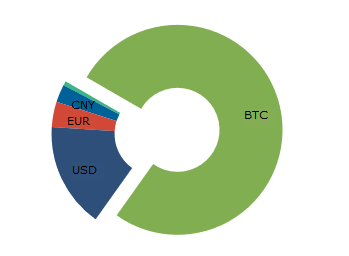
\includegraphics[scale=1]{Appendix/Volume}\medbreak
\caption{ETH Exchange Volume by Currency - November 2016} \cite{CRYPTOCOMPARE}
\label{VOLUME}
\end{figure}

\clearpage
\section*{Chapter 2}
\subsection*{DF-GLS TEST}
\begin{figure}[!h]
\begin{minipage}[c]{.46\linewidth}
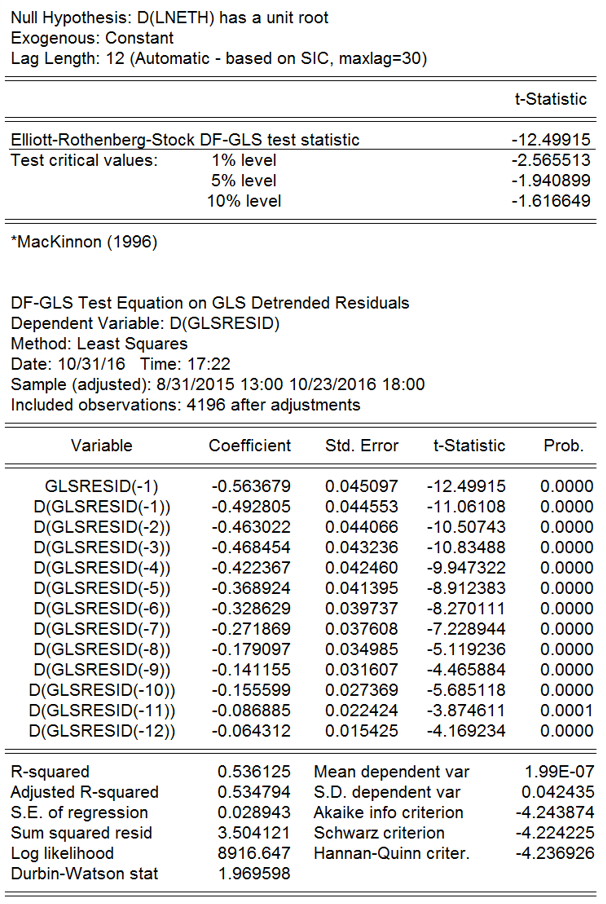
\includegraphics[scale=0.5]{Appendix/chap2/1}
\end{minipage} \hfill
\begin{minipage}[c]{.46\linewidth}
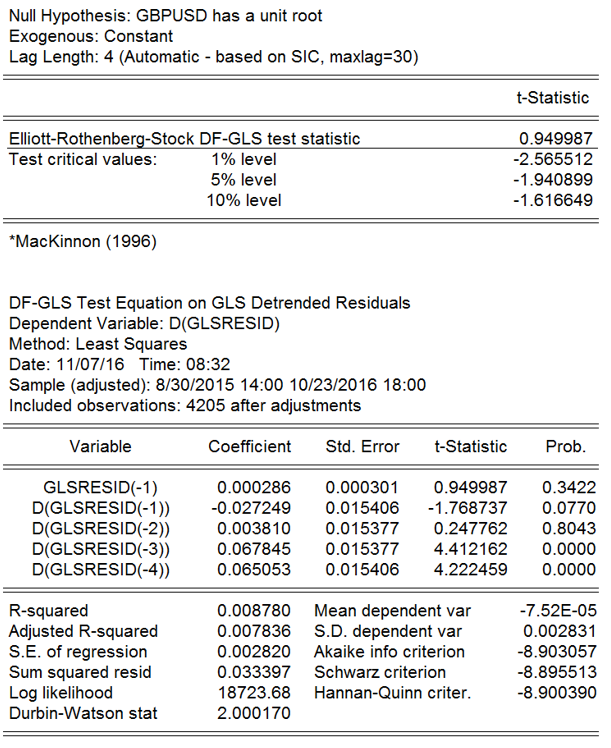
\includegraphics[scale=0.5]{Appendix/chap2/2}
\end{minipage} \hfill
\end{figure}
\begin{figure}[!h]
\begin{minipage}[c]{.46\linewidth}
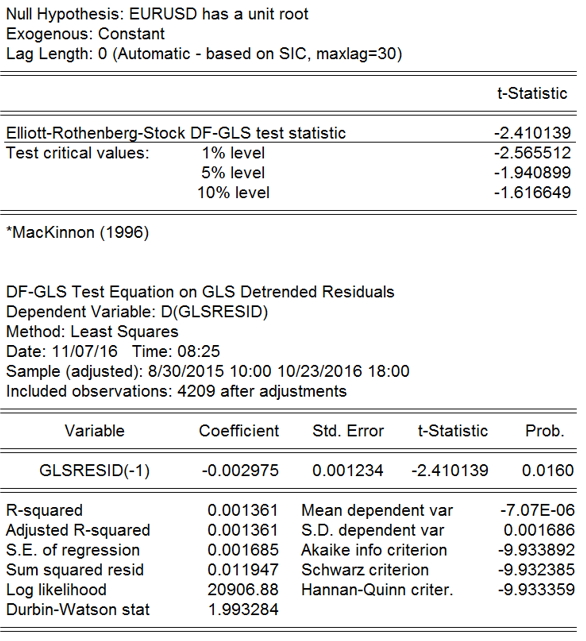
\includegraphics[scale=0.5]{Appendix/chap2/3}
\end{minipage} \hfill
\begin{minipage}[c]{.46\linewidth}
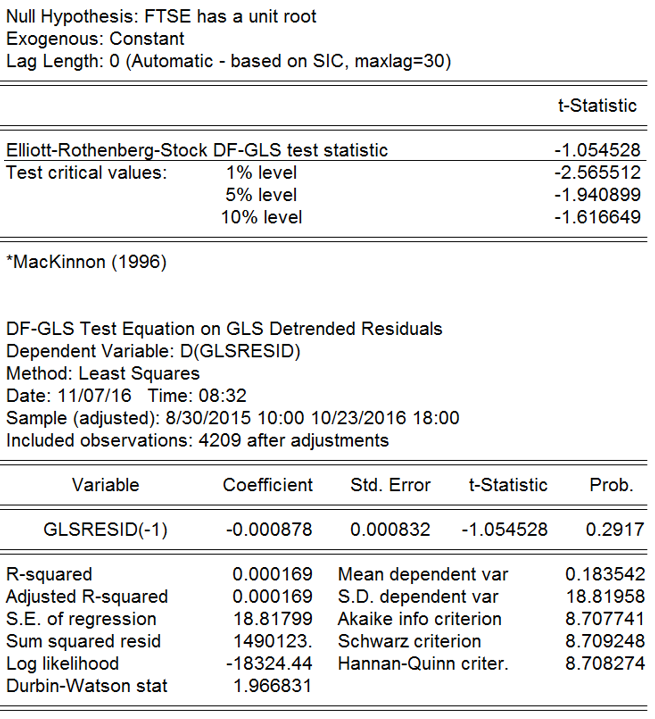
\includegraphics[scale=0.5]{Appendix/chap2/4}
\end{minipage} \hfill
\end{figure}
\begin{figure}[!h]
\begin{minipage}[c]{.46\linewidth}
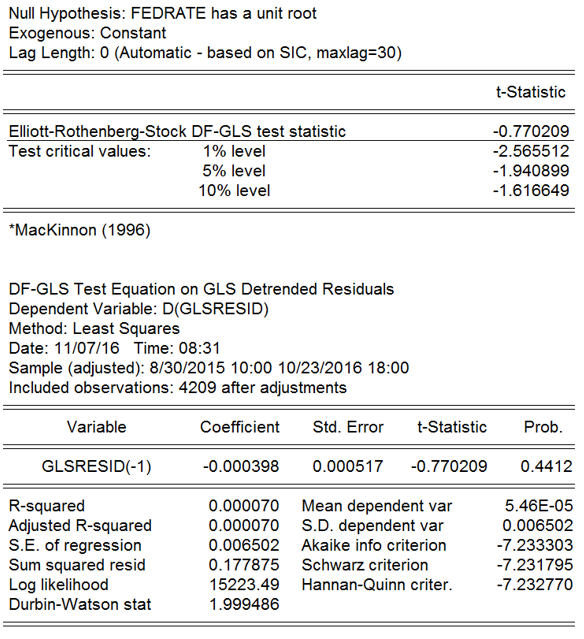
\includegraphics[scale=0.5]{Appendix/chap2/5}
\end{minipage} \hfill
\begin{minipage}[c]{.46\linewidth}
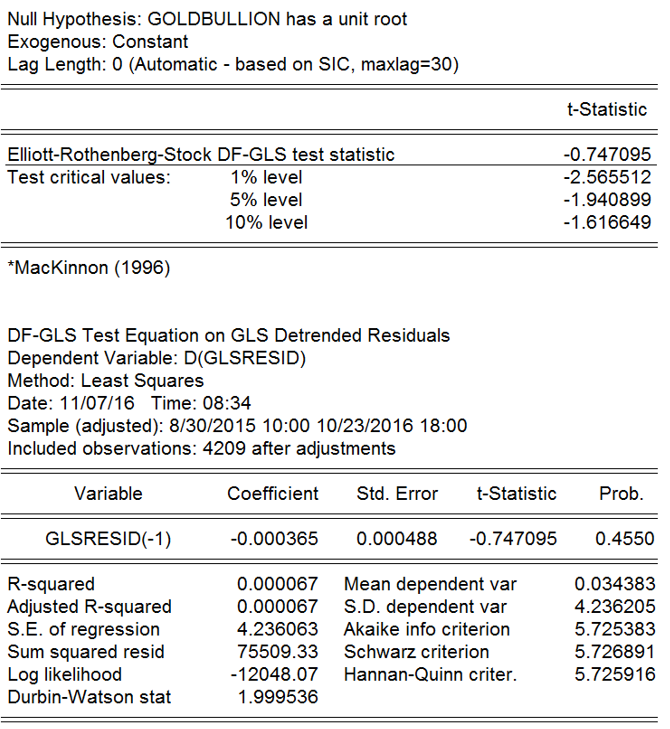
\includegraphics[scale=0.5]{Appendix/chap2/6}
\end{minipage} \hfill
\end{figure}
\begin{figure}[!h]
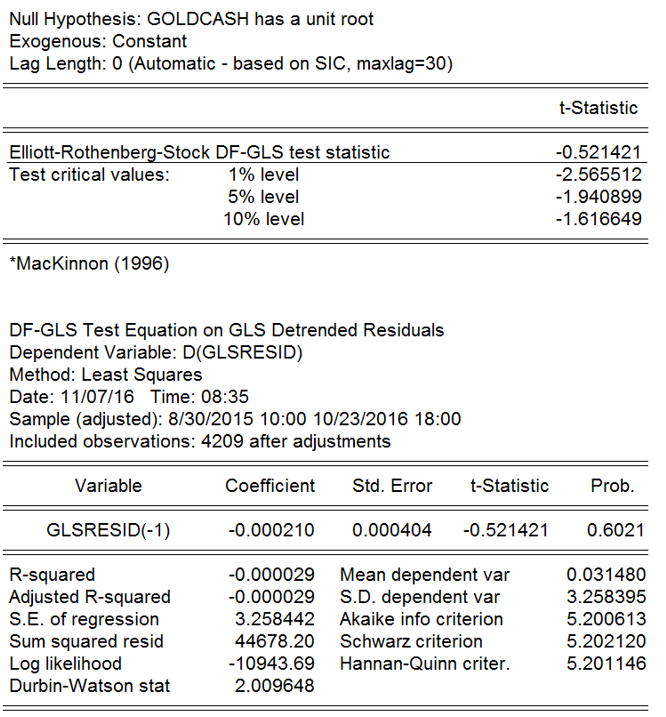
\includegraphics[scale=0.5]{Appendix/chap2/7}
\end{figure}
\clearpage

\subsection*{KPSS test - Unit roots}
\begin{figure}[!h]
\begin{minipage}[c]{.46\linewidth}
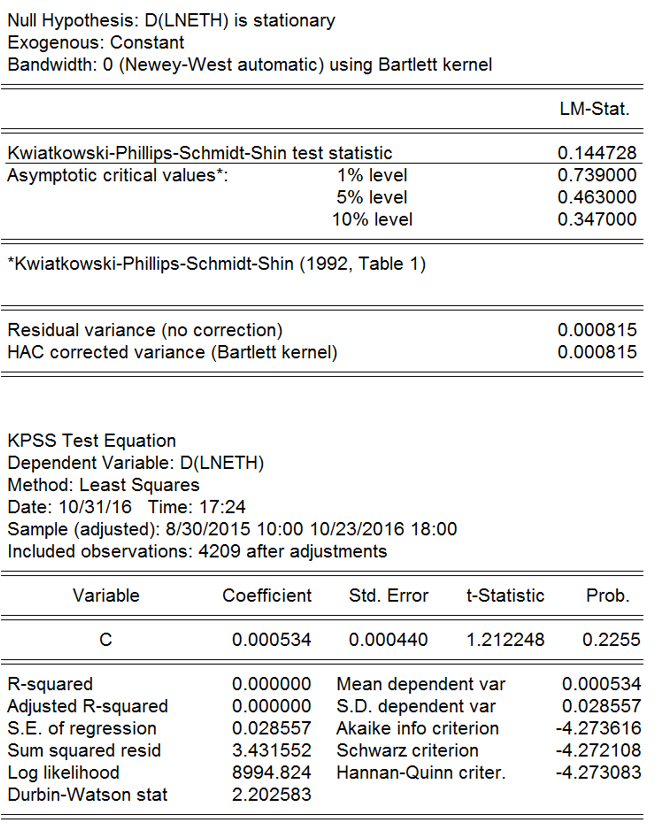
\includegraphics[scale=0.5]{Appendix/chap2/8}
\end{minipage} \hfill
\begin{minipage}[c]{.46\linewidth}
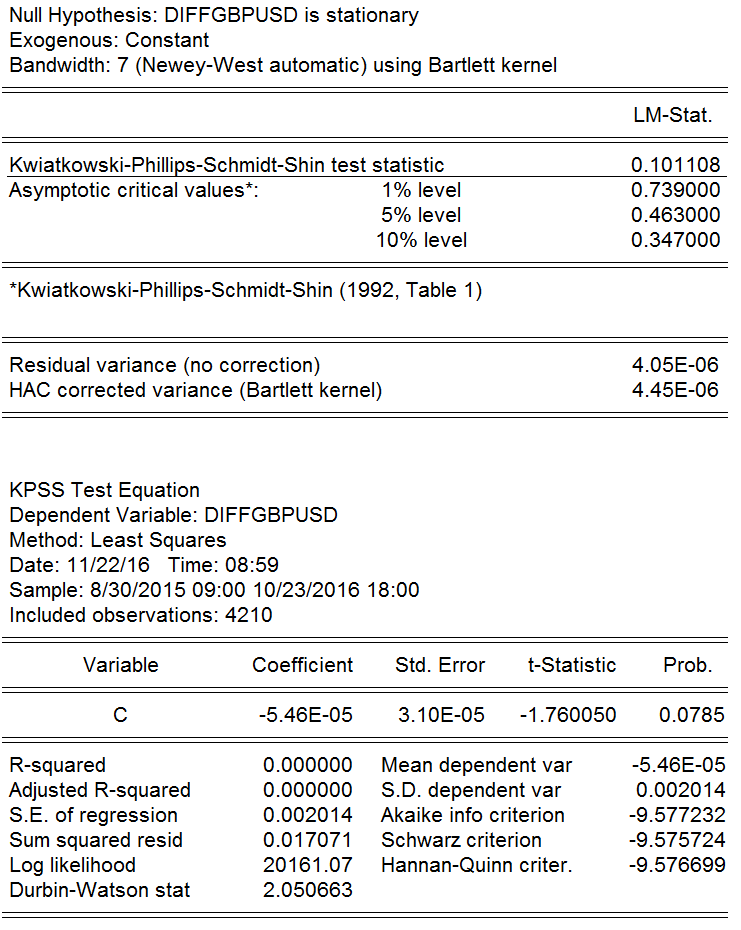
\includegraphics[scale=0.5]{Appendix/chap2/9}
\end{minipage} \hfill
\end{figure}
\begin{figure}[!h]
\begin{minipage}[c]{.46\linewidth}
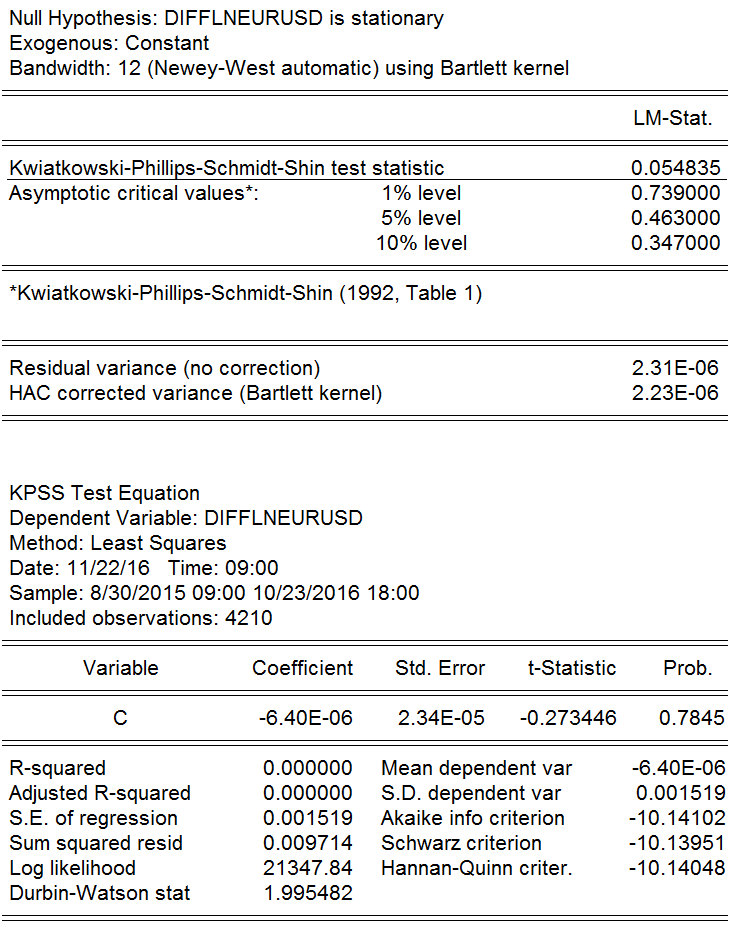
\includegraphics[scale=0.5]{Appendix/chap2/10}
\end{minipage} \hfill
\begin{minipage}[c]{.46\linewidth}
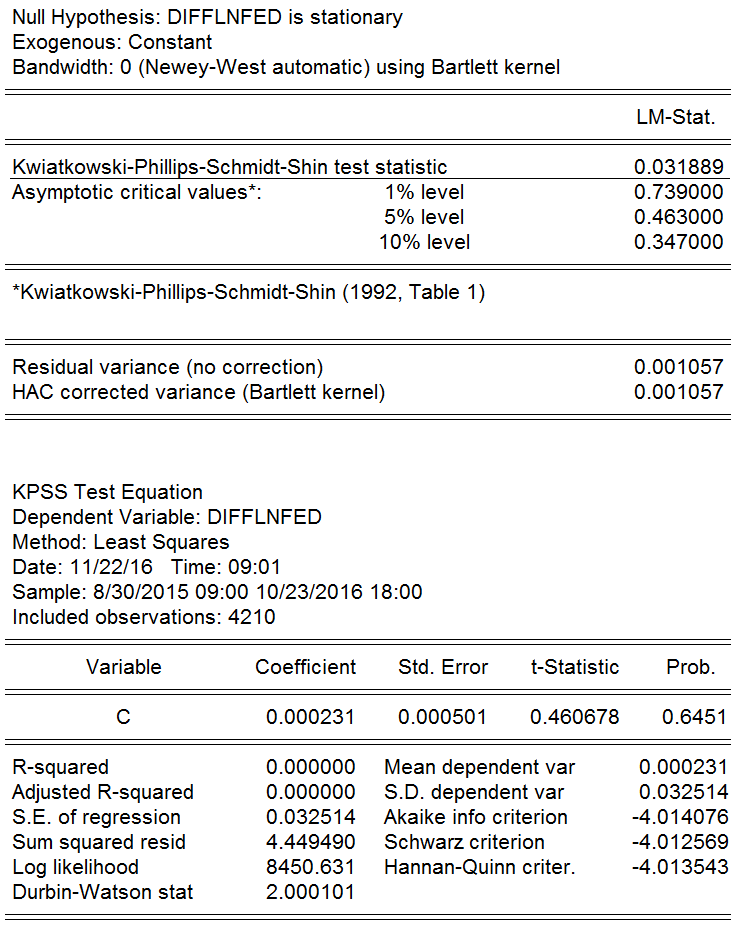
\includegraphics[scale=0.5]{Appendix/chap2/11}
\end{minipage} \hfill
\end{figure}
\begin{figure}[!h]
\begin{minipage}[c]{.46\linewidth}
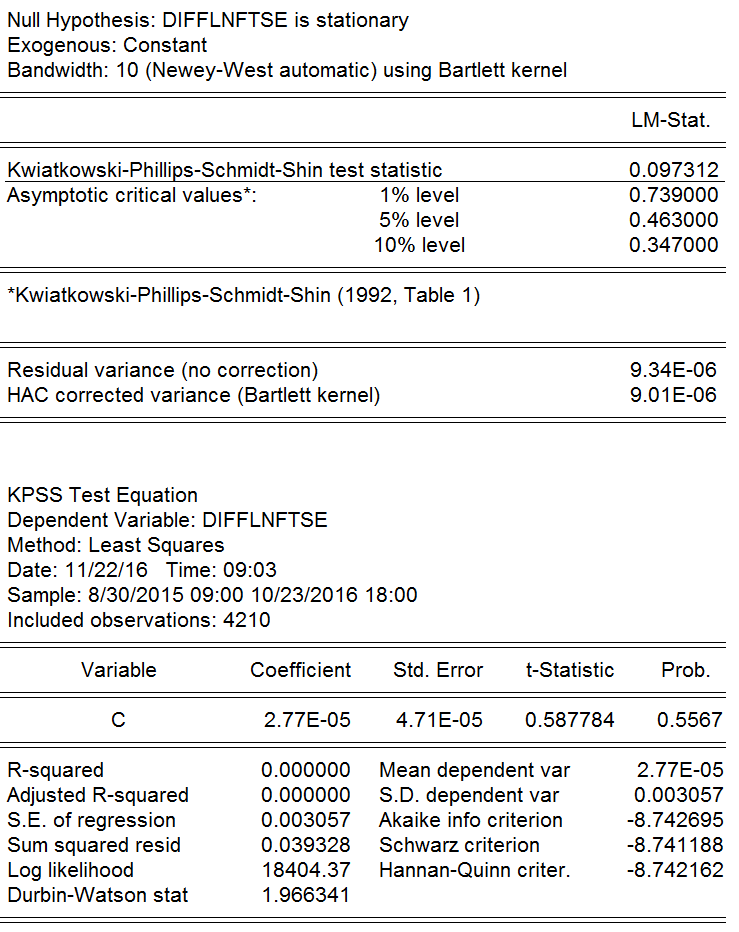
\includegraphics[scale=0.5]{Appendix/chap2/12}
\end{minipage} \hfill
\begin{minipage}[c]{.46\linewidth}
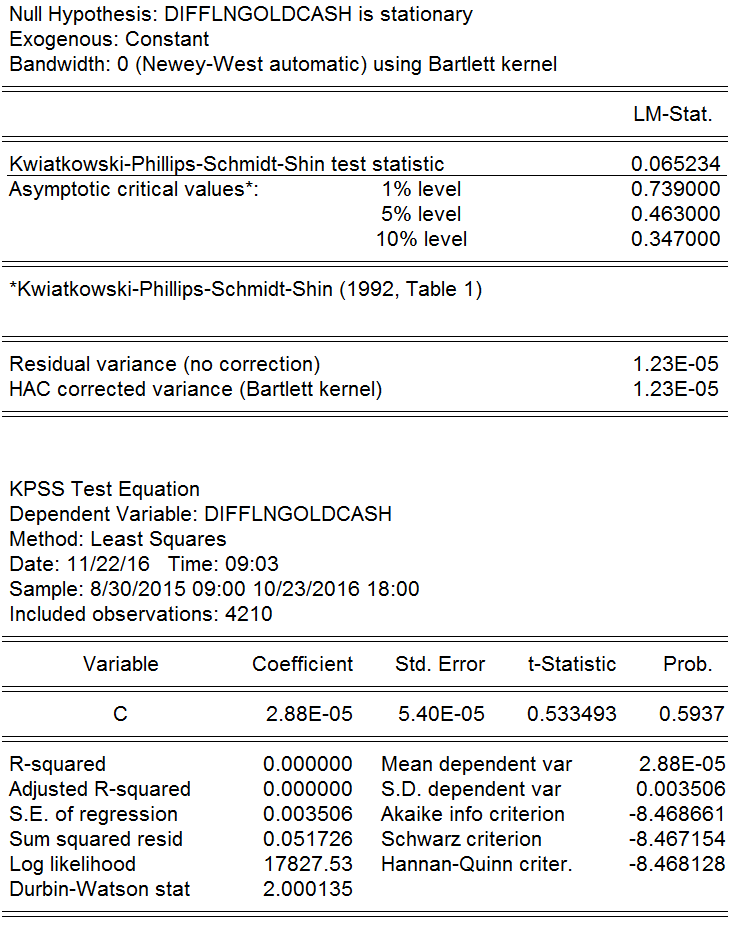
\includegraphics[scale=0.5]{Appendix/chap2/13}
\end{minipage} \hfill
\end{figure}
\begin{figure}[!h]
\centering
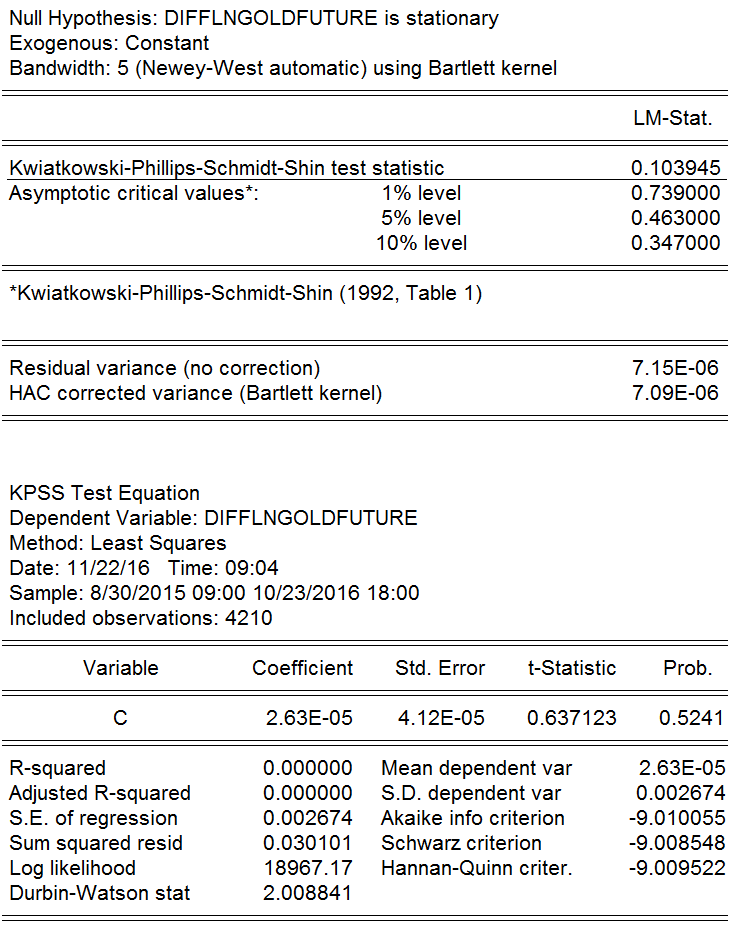
\includegraphics[scale=0.5]{Appendix/chap2/14}
\end{figure}
\clearpage

\subsection*{Test for Arch effects}
\subsubsection*{Heteroskedasticity test}
\begin{figure}[!h]
\centering
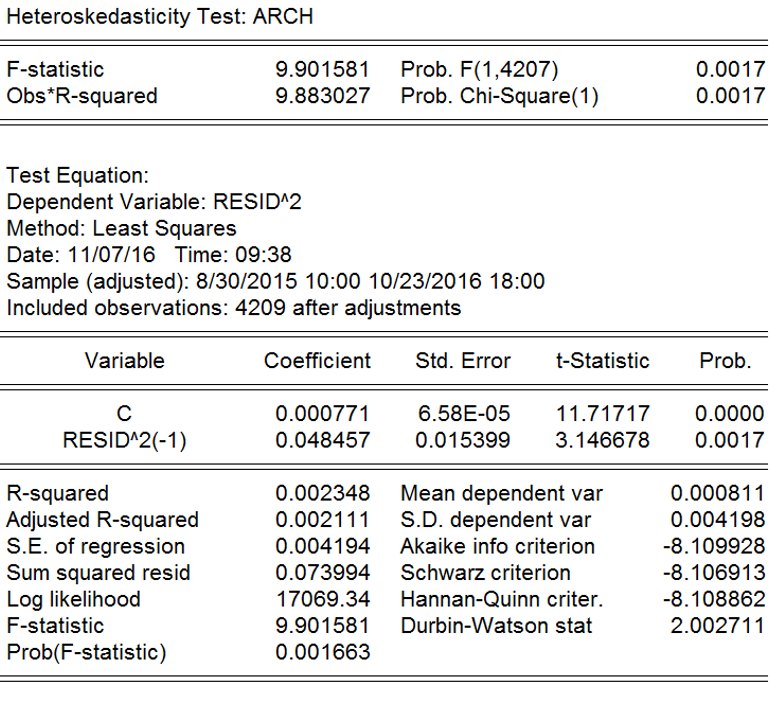
\includegraphics[scale=0.5]{Appendix/chap2/15}
\end{figure}
\begin{figure}[!h]
\centering
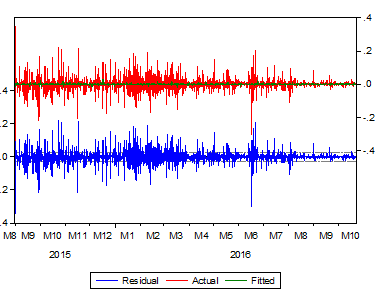
\includegraphics[scale=1.5]{Appendix/chap2/16}
\end{figure}
\clearpage
\subsubsection*{Hypothesis of autocorrelation}
\begin{figure}[!h]
\centering
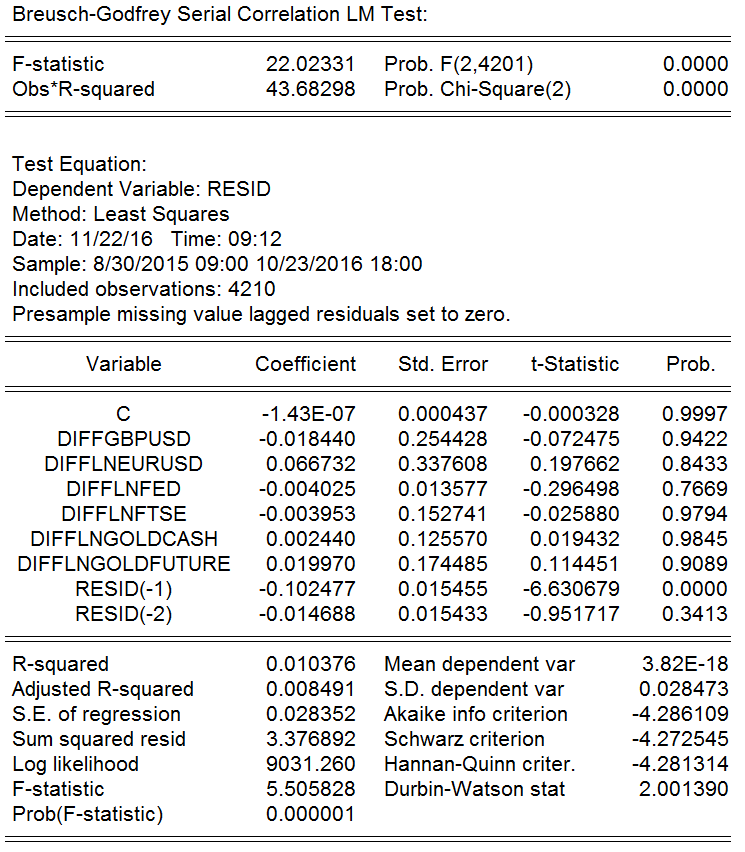
\includegraphics[scale=0.5]{Appendix/chap2/17}
\end{figure}
\clearpage
\subsubsection*{Hypothesis of normality of errors}
\begin{figure}[!h]
\centering
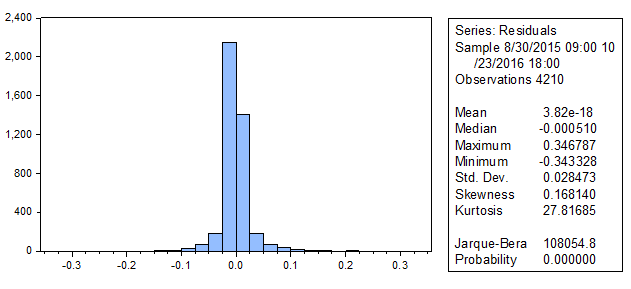
\includegraphics[scale=1.5]{Appendix/chap2/18}
\end{figure}
\clearpage
\subsection*{GARCH Analysis}
\begin{figure}[!h]
\centering
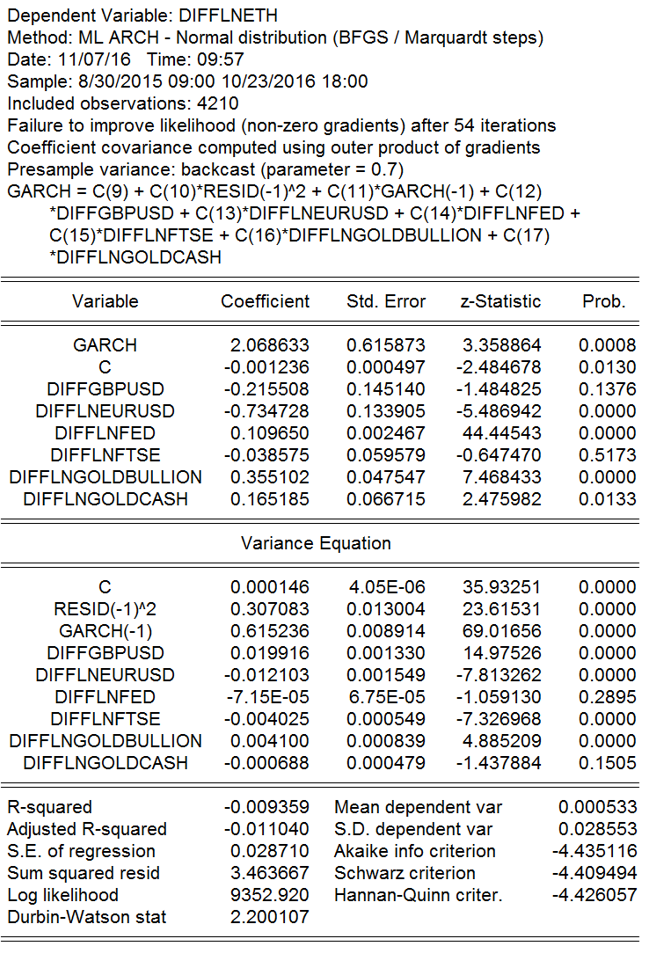
\includegraphics[scale=0.6]{Appendix/chap2/19}
\end{figure}
\clearpage
\section*{Chapter 3}
\subsection*{Hedge against the FTSE index}
\subsubsection*{Heteroskedasticity test}
\begin{figure}[!h]
\centering
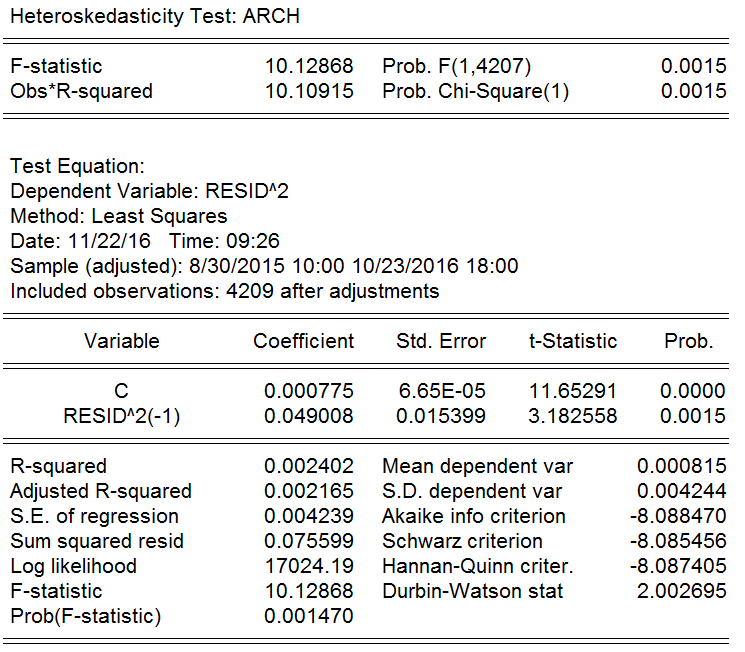
\includegraphics[scale=0.5]{Appendix/chap3/1}
\end{figure}
\begin{figure}[!h]
\centering
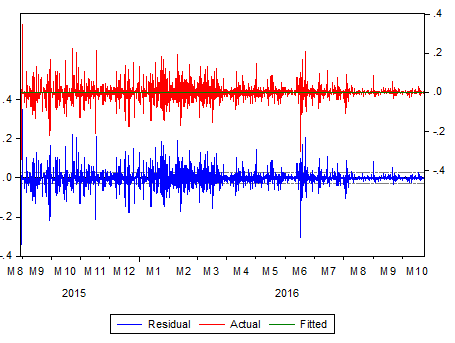
\includegraphics[scale=1]{Appendix/chap3/2}
\end{figure}
\clearpage
\subsubsection*{Hypothesis of autocorrelation}
\begin{figure}[!h]
\centering
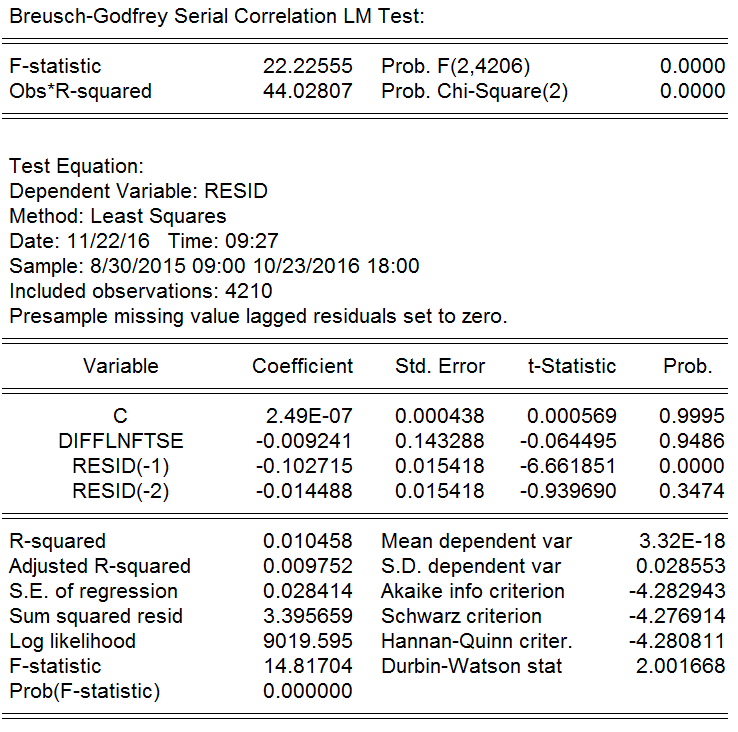
\includegraphics[scale=0.5]{Appendix/chap3/3}
\end{figure}
\subsubsection*{Hypothesis of normality of errors}
\begin{figure}[!h]
\centering
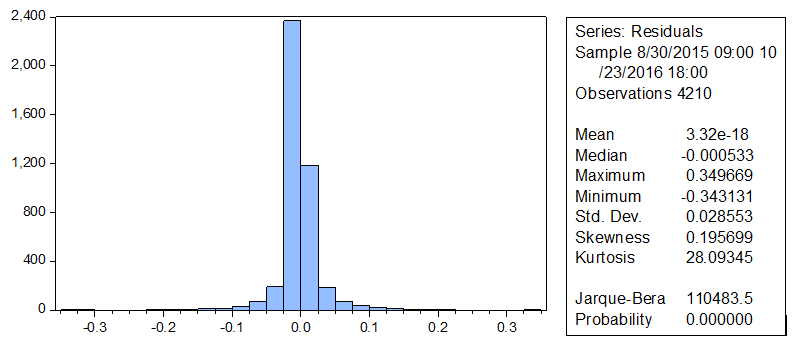
\includegraphics[scale=1]{Appendix/chap3/4}
\end{figure}
\clearpage
\subsubsection*{GARCH Analysis}
\begin{figure}[!h]
\centering
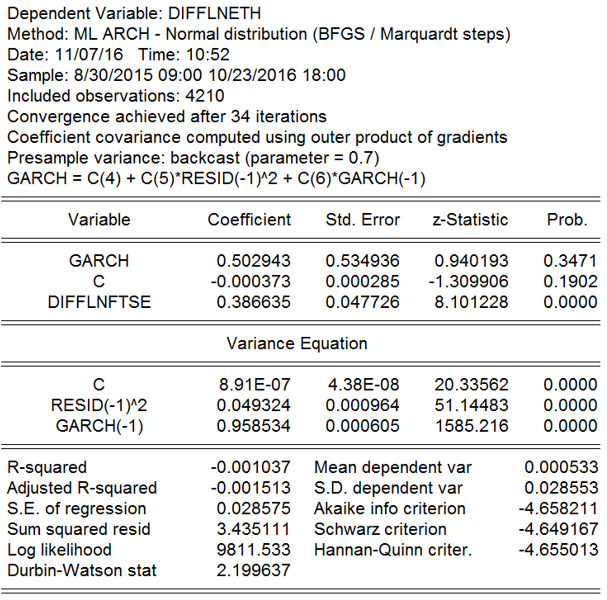
\includegraphics[scale=0.6]{Appendix/chap3/5}
\end{figure}
\clearpage
\subsection*{Hedge against the Dollar}
\subsubsection*{Heteroskedasticity test}
\textbf{EUR-USD Exchange rate}
\begin{figure}[!h]
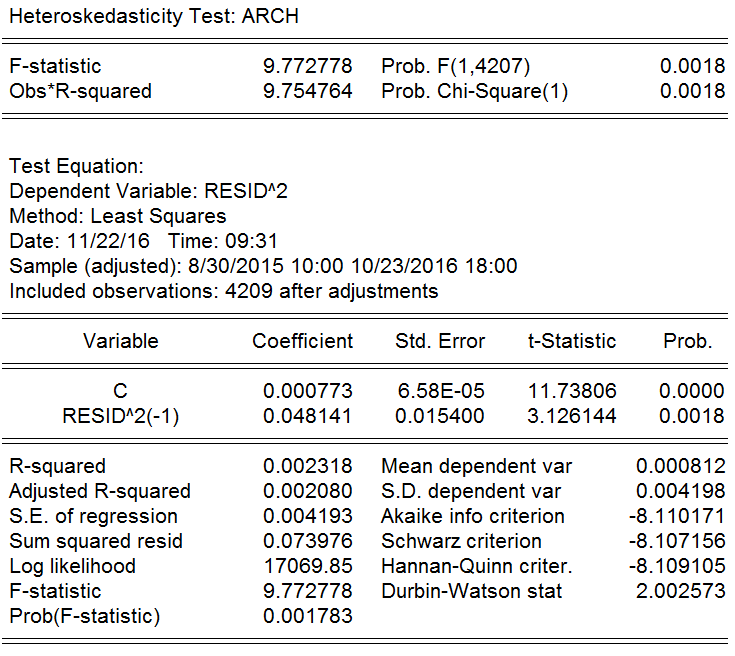
\includegraphics[scale=0.5]{Appendix/chap3/6}
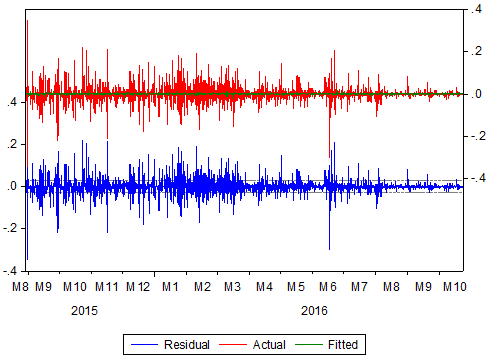
\includegraphics[scale=1]{Appendix/chap3/7}
\end{figure}
\smallbreak
\textbf{GBP-USD Exchange rate}
\begin{figure}[!h]
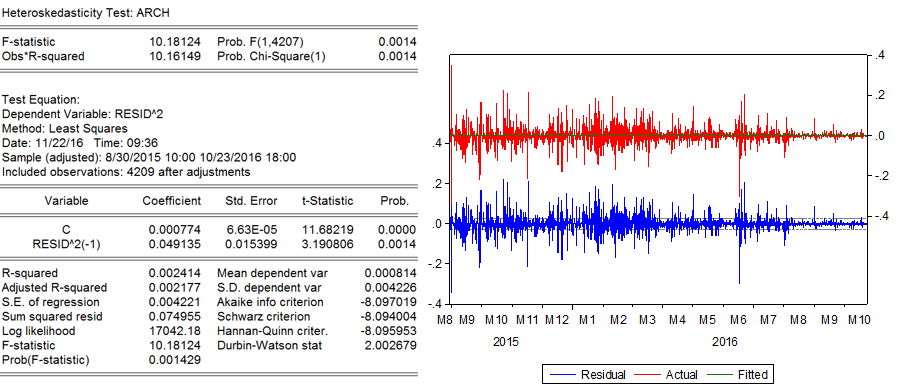
\includegraphics[scale=1.2]{Appendix/chap3/8}
\end{figure}
\clearpage

\subsubsection*{Hypothesis of autocorrelation}
\textbf{EUR-USD exchange rate and GBP-USD exchange rate}
\begin{figure}[!h]
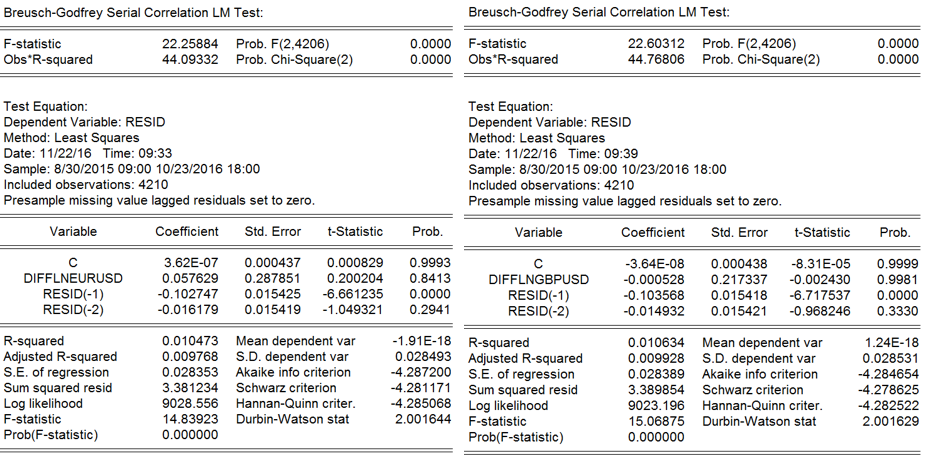
\includegraphics[scale=1.1]{Appendix/chap3/10}
\end{figure}
\clearpage

\subsubsection*{Hypothesis of normality of errors}
\textbf{EUR-USD exchange rate}
\begin{figure}[!h]
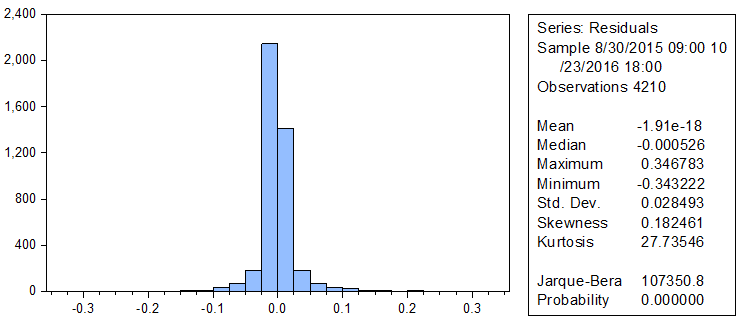
\includegraphics[scale=1.2]{Appendix/chap3/11}
\end{figure}
\smallbreak
\textbf{GBP-USD exchange rate }
\begin{figure}[!h]
\includegraphics[scale=1.2]{Appendix/chap3/12}
\end{figure}
\clearpage
\subsection*{GARCH Analysis}
\textbf{EUR-USD exchange rate and GBP-USD exchange rate}
\begin{figure}[!h]
\includegraphics[scale=1.1]{Appendix/chap3/13}
\end{figure}
\clearpage

\section*{Chapter 4}
\subsection*{Bitcoin and Ether's price correlation}
\begin{figure}[!h]
\centering
\includegraphics[scale=0.5]{Chap5/Variation}\medbreak
\centering
\caption{ETH/USD \& BTC/USD variation}
\label{Variation}
\end{figure}

Correlation results based on Pearson's $r$ on IBM SPSS - Daily data from November 2015 to November 2016 - : \medbreak

\begin{figure}[!h]
\centering
\includegraphics[scale=0.8]{Chap5/CorrelationETHUSDBTCUSD}\medbreak
\caption{ETH/USD \& BTC/USD Correlation}
\label{Correlation}
\end{figure}

\subsection*{Ethereum's visibility impact on Ether's price}

\begin{figure}[!h]
\centering
\includegraphics[scale=0.7]{Chap5/VIF}
\medbreak
\caption{Multicollinearity Results}
\label{VIF}
\end{figure}

\clearpage
\section*{Chapter 5}
\subsection*{Traditional Event Analysis}
\begin{table}[!h]
\centering
\begin{tabular}{c|c|c|c|c|c|c|}
\cline{2-7}
                                          & AR ETH          & T-stat AR        & Signifiance test & CAR ETH          & T-stat CAR       & Signifiance test \\ \hline
\multicolumn{1}{|c|}{07/06/2016}          & 0,0149          & 0,175            & No               & 0,0149           & 0,175            & No               \\ \hline
\multicolumn{1}{|c|}{08/06/2016}          & -0,0165         & -0,1939          & No               & -0,0016          & -0,0188          & No               \\ \hline
\multicolumn{1}{|c|}{09/06/2016}          & -0,0182         & -0,2135          & No               & -0,0198          & -0,2323          & No               \\ \hline
\multicolumn{1}{|c|}{10/06/2016}          & -0,051          & -0,5978          & No               & -0,0709          & -0,8301          & No               \\ \hline
\multicolumn{1}{|c|}{11/06/2016}          & -0,0062         & -0,0725          & No               & -0,077           & -0,9026          & No               \\ \hline
\multicolumn{1}{|c|}{12/06/2016}          & 0,1031          & 1,2076           & No               & 0,026            & 0,305            & No               \\ \hline
\multicolumn{1}{|c|}{13/06/2016}          & 0,1127          & 1,3198           & No               & 0,1387           & 1,6248           & No               \\ \hline
\multicolumn{1}{|c|}{14/06/2016}          & 0,0418          & 0,49             & No               & 0,1805           & 2,1148           & Yes              \\ \hline
\multicolumn{1}{|c|}{15/06/2016}          & -0,0336         & -0,3936          & No               & 0,1469           & 1,7212           & No               \\ \hline
\multicolumn{1}{|c|}{16/06/2016}          & 0,1219          & 1,428            & No               & 0,2688           & 3,1491           & Yes              \\ \hline
\multicolumn{1}{|c|}{\textbf{17/06/2016}} & \textbf{-0,278} & \textbf{-3,2566} & \textbf{Yes}     & \textbf{-0,0092} & \textbf{-0,1075} & \textbf{No}      \\ \hline
\multicolumn{1}{|c|}{18/06/2016}          & -0,2746         & -3,2171          & Yes              & -0,2838          & -3,3246          & Yes              \\ \hline
\multicolumn{1}{|c|}{19/06/2016}          & 0,065           & 0,7609           & No               & -0,2188          & -2,5637          & Yes              \\ \hline
\multicolumn{1}{|c|}{20/06/2016}          & -0,0641         & -0,7506          & No               & -0,2829          & -3,3142          & Yes              \\ \hline
\multicolumn{1}{|c|}{21/06/2016}          & 0,0601          & 0,7037           & No               & -0,2228          & -2,6105          & Yes              \\ \hline
\multicolumn{1}{|c|}{22/06/2016}          & -0,0025         & -0,0297          & No               & -0,2254          & -2,6402          & Yes              \\ \hline
\multicolumn{1}{|c|}{23/06/2016}          & 0,0267          & 0,3132           & No               & -0,1986          & -2,327           & Yes              \\ \hline
\multicolumn{1}{|c|}{24/06/2016}          & 0,0312          & 0,3657           & No               & -0,1674          & -1,9613          & Yes              \\ \hline
\multicolumn{1}{|c|}{25/06/2016}          & -0,0125         & -0,1465          & No               & -0,1799          & -2,1078          & Yes              \\ \hline
\multicolumn{1}{|c|}{26/06/2016}          & -0,0621         & -0,727           & No               & -0,242           & -2,8348          & Yes              \\ \hline
\multicolumn{1}{|c|}{27/06/2016}          & 0,0007          & 0,0086           & No               & -0,2412          & -2,8262          & Yes              \\ \hline
\multicolumn{1}{|c|}{28/06/2016}          & -0,1543         & -1,8074          & No               & -0,3955          & -4,6336          & Yes              \\ \hline
\multicolumn{1}{|c|}{29/06/2016}          & 0,0521          & 0,6104           & No               & -0,3434          & -4,0232          & Yes              \\ \hline
\multicolumn{1}{|c|}{30/06/2016}          & -0,0478         & -0,5598          & No               & -0,3912          & -4,583           & Yes              \\ \hline
\multicolumn{1}{|c|}{01/07/2016}          & -0,0288         & -0,3378          & No               & -0,42            & -4,9208          & Yes              \\ \hline
\multicolumn{1}{|c|}{02/07/2016}          & -0,0314         & -0,3684          & No               & -0,4515          & -5,2892          & Yes              \\ \hline
\multicolumn{1}{|c|}{03/07/2016}          & -0,0394         & -0,4612          & No               & -0,4909          & -5,7504          & Yes              \\ \hline
\multicolumn{1}{|c|}{04/07/2016}          & -0,057          & -0,6683          & No               & -0,5479          & -6,4186          & Yes              \\ \hline
\multicolumn{1}{|c|}{05/07/2016}          & -0,1085         & -1,271           & No               & -0,6564          & -7,6896          & Yes              \\ \hline
\multicolumn{1}{|c|}{06/07/2016}          & -0,0026         & -0,0307          & No               & -0,659           & -7,7203          & Yes              \\ \hline
\multicolumn{1}{|c|}{07/07/2016}          & -0,0671         & -0,7864          & No               & -0,7261          & -8,5067          & Yes              \\ \hline
\multicolumn{1}{|c|}{08/07/2016}          & 0,1059          & 1,2408           & No               & -0,6202          & -7,2659          & Yes              \\ \hline
\multicolumn{1}{|c|}{09/07/2016}          & -0,0473         & -0,5542          & No               & -0,6675          & -7,8202          & Yes              \\ \hline
\multicolumn{1}{|c|}{10/07/2016}          & -0,016          & -0,1877          & No               & -0,6836          & -8,0079          & Yes              \\ \hline
\multicolumn{1}{|c|}{11/07/2016}          & -0,0522         & -0,6118          & No               & -0,7358          & -8,6197          & Yes              \\ \hline
\end{tabular}
\end{table}
\clearpage
\begin{table}[]
\centering
\begin{tabular}{c|c|c|c|c|c|c|}
\cline{2-7}
                                          & AR ETH          & T-stat AR       & Signifiance test & CAR ETH          & T-stat CAR       & Signifiance test \\ \hline
\multicolumn{1}{|c|}{12/07/2016}          & -0,015          & -0,1759         & No               & -0,7508          & -8,7955          & Yes              \\ \hline
\multicolumn{1}{|c|}{13/07/2016}          & -0,0265         & -0,3109         & No               & -0,7773          & -9,1065          & Yes              \\ \hline
\multicolumn{1}{|c|}{14/07/2016}          & 0,0827          & 0,9688          & No               & -0,6946          & -8,1377          & Yes              \\ \hline
\multicolumn{1}{|c|}{15/07/2016}          & 0,0242          & 0,2833          & No               & -0,6705          & -7,8544          & Yes              \\ \hline
\multicolumn{1}{|c|}{16/07/2016}          & -0,0436         & -0,5111         & No               & -0,7141          & -8,3654          & Yes              \\ \hline
\multicolumn{1}{|c|}{17/07/2016}          & -0,0522         & -0,6121         & No               & -0,7663          & -8,9775          & Yes              \\ \hline
\multicolumn{1}{|c|}{18/07/2016}          & -0,0367         & -0,43           & No               & -0,803           & -9,4075          & Yes              \\ \hline
\multicolumn{1}{|c|}{19/07/2016}          & 0,0442          & 0,5179          & No               & -0,7588          & -8,8896          & Yes              \\ \hline
\multicolumn{1}{|c|}{20/07/2016}          & 0,0508          & 0,5951          & No               & -0,708           & -8,2945          & Yes              \\ \hline
\multicolumn{1}{|c|}{21/07/2016}          & -0,011          & -0,1294         & No               & -0,7191          & -8,424           & Yes              \\ \hline
\multicolumn{1}{|c|}{\textbf{22/07/2016}} & \textbf{0,1543} & \textbf{1,8078} & \textbf{No}      & \textbf{-0,5648} & \textbf{-6,6162} & \textbf{Yes}     \\ \hline
\multicolumn{1}{|c|}{23/07/2016}          & -0,0491         & -0,5746         & No               & -0,6138          & -7,1908          & Yes              \\ \hline
\multicolumn{1}{|c|}{24/07/2016}          & -0,1319         & -1,5451         & No               & -0,7457          & -8,7359          & Yes              \\ \hline
\multicolumn{1}{|c|}{25/07/2016}          & 0,0701          & 0,8217          & No               & -0,6756          & -7,9141          & Yes              \\ \hline
\multicolumn{1}{|c|}{26/07/2016}          & -0,1401         & -1,6407         & No               & -0,8156          & -9,5548          & Yes              \\ \hline
\multicolumn{1}{|c|}{27/07/2016}          & 0,0638          & 0,747           & No               & -0,7518          & -8,8078          & Yes              \\ \hline
\multicolumn{1}{|c|}{28/07/2016}          & -0,0335         & -0,3926         & No               & -0,7854          & -9,2004          & Yes              \\ \hline
\multicolumn{1}{|c|}{29/07/2016}          & -0,0163         & -0,1914         & No               & -0,8017          & -9,3918          & Yes              \\ \hline
\multicolumn{1}{|c|}{30/07/2016}          & -0,045          & -0,5266         & No               & -0,8466          & -9,9184          & Yes              \\ \hline
\multicolumn{1}{|c|}{31/07/2016}          & -0,0715         & -0,8374         & No               & -0,9181          & -10,7558         & Yes              \\ \hline
\multicolumn{1}{|c|}{01/08/2016}          & -0,0886         & -1,0375         & No               & -1,0067          & -11,7933         & Yes              \\ \hline
\end{tabular}
\end{table}
\end{document}
